%%%%%%%%%%%%%%%%%%%%%%%%%%%%%%%%%%%%%%%%%%%%%%%%%%%%%%%%%%%%%%%%%%%%%%%%
% Plantilla TFG/TFM
% Escuela Politécnica Superior de la Universidad de Alicante
% Realizado por: Jose Manuel Requena Plens
% Contacto: info@jmrplens.com / Telegram:@jmrplens
%%%%%%%%%%%%%%%%%%%%%%%%%%%%%%%%%%%%%%%%%%%%%%%%%%%%%%%%%%%%%%%%%%%%%%%%

\chapter{Desarrollo}
\label{desarrollo}
\section{Requisitos}
\label{requisitos}
En esta sección realizaremos una toma de los requisitos generales del sistema, seguidos de requisitos específicos.
\subsection{Funcionales}
Los requisitos funcionales son especificaciones que definen las funciones o características que un sistema debe poseer. Estos describen el comportamiento del sistema bajo ciertas condiciones y definen lo que el sistema debe hacer.

\subsubsection{Generales}
\begin{itemize}
    \item \textbf{R1:} Cada uno de los usuarios tendrá acceso a una información específica, pudiendo acceder solamente a los datos y funciones a los que tenga permiso ver.
    
    \item \textbf{R2:} Se podrán generar informes de rendimiento para los jugadores y el equipo técnico.
    
    \item \textbf{R3:} Cada entrenador de una organización podrá acceder a la información de todos los actores que forman parte de la organización.
    
    \item \textbf{R4:} Los entrenadores tendrán acceso a todas las sesiones de entrenamiento y a estadísticas individuales y grupales de cada jugador.    
\end{itemize}

\subsubsection{Entrenamientos}
\begin{itemize}
    \item \textbf{R5:} Los usuarios tendrán un apartado para acceder a un calendario, que mostrará cada sesión.
    \item \textbf{R6:} Para cada sesión, se mostrará específicamente el nombre de ésta, el día y la hora de inicio y fin de la sesión.
\end{itemize}

\subsubsection{Seguimiento y Evaluación del Rendimiento}
\begin{itemize}
    \item \textbf{R7:} Evaluar el rendimiento de los jugadores mediante la recolección de estadísticas durante los entrenamientos y partidos.
    
    \item \textbf{R8:} Mostrar el historial de puntuaciones dadas por el entrenador por cada intervalo de  tiempo definido.
    
    \item \textbf{R9:} Elaborar gráficos de las puntuaciones de los KPIs para todo el equipo para que se pueda apreciar la evolución del equipo en un conjunto.
    
    \item \textbf{R10:} Elaborar gráficos de las puntuaciones de los KPIs para cada jugador, pudiendo apreciarse la evolución individual.
    
    \item \textbf{R11:} Desarrollar un algoritmo estadístico para generar una matriz DAFO (debilidades, Amenazas, Fortalezas y Debilidades) que permitan al entrenador analizar de una manera más precisa las necesidades de sus jugadores.
    
\end{itemize}

\subsubsection{Equipo}
\begin{itemize}
    \item \textbf{R12:} El entrenador podrá ver toda la información detallada del equipo
    
    \item \textbf{R13:} El entrenador podrá ver toda la información detallada de cada jugador individualmente
    
\end{itemize}

\subsubsection{Intervalos de tiempo}
\begin{itemize}
    \item \textbf{R14:} Los usuarios podrán acceder a un histórico de los datos en un intervalo de tiempo correspondiente a una sesión.
    
    \item \textbf{R15:} Los usuarios podrán acceder a un histórico de los datos en un intervalo de tiempo correspondiente a un mes.
    
    \item \textbf{R16:} Los usuarios podrán acceder a un histórico de los datos en un intervalo de tiempo correspondiente a un trimestre.
    
\end{itemize}

\subsubsection{Actores}
\begin{itemize}
    \item \textbf{R17:} Los entrenadores podrán acceder a la información de los actores que componen la organización.
    
    \item \textbf{R18:} Cada ventana del actor tendrá su información correspondiente al seguimiento de dicho actor.
    
\end{itemize}

\subsection{No Funcionales}
Los requisitos no funcionales describen cómo el sistema debe comportarse. Estos incluyen aspectos como el rendimiento, la seguridad, la usabilidad, la escalabilidad y la disponibilidad del sistema.

\subsubsection{Rendimiento}
\begin{itemize}
    \item \textbf{Capacidad de carga:} La plataforma debe ser capaz de manejar una cantidad considerable de usuarios simultáneos sin afectar al rendimiento.
    
    \item \textbf{Tiempo de Respuesta:} La carga de los datos debe completarse en un tiempo rápido.
    
    \item \textbf{Optimización:} Las consultas a la base de datos deben de estar optimizadas para minimizar el tiempo de espera.
    
\end{itemize}

\subsubsection{Seguridad}
\begin{itemize}
    \item \textbf{Autenticación:} Las operaciones de carga de datos no se realizarán hasta que el usuario no se haya autenticado correctamente.
    
    \item \textbf{Protección de datos:} Los datos personales de los usuarios deben ser almacenados y procesados conforme a las normativas de protección de datos.
    
\end{itemize}

\subsubsection{Facilidad de uso}
\begin{itemize}
    \item \textbf{Interfaz intuitiva:} La interfaz de usuario debe ser intuitiva y fácil de usar, permitiendo a los usuarios utilizar la plataforma desde cero sin tener que formarse para ello.
    
    \item \textbf{Documentación:} Los usuarios deben poder acceder a una documentación clara para usar la plataforma.
    
\end{itemize}

\subsubsection{Escalabilidad}
\begin{itemize}
    \item \textbf{Escalabilidad horizontal:} La plataforma debe poder escalar horizontalmente (añadiendo mas servidores) para reducir la carga de éstos y mejorar la experiencia del usuario.
    
    \item \textbf{Escalabilidad vertical:} La plataforma debe poder escalar verticalmente (mejorando los servidores) para manejar el aumento de usuarios y la carga de trabajo.
    
\end{itemize}

\subsubsection{Compatibilidad}
\begin{itemize}
    \item \textbf{Multiplataforma:} La plataforma ser accesible en distintos sistemas operativos, así como desde diferentes tipos de dispositivo (móvil u ordenadores).
    
\end{itemize}

\subsubsection{Fiabilidad}
\begin{itemize}
    \item \textbf{Tolerancia a fallos:} El sistema debe manejar los errores de una manera adecuada, proporcionando mensajes de error claros para su rápida resolución.
    
    \item \textbf{Consistencia de datos:} Los datos deben mantenerse consistentes y libres de errores.
    
\end{itemize}

\section{Análisis funcional del sistema}
\subsection{Historias de usuario}
Para la gestión ágil de este proyecto, comenzaremos a describir historias de usuario. Siguiendo una estructura sistemática para reflejar las necesidades de los usuarios que se traducen en requisitos funcionales para el sistema que influirán en el diseño y desarrollo de la plataforma.

%----------------Iniciar Sesión------------------------
\begin{tcolorbox}[title= Inicio de sesión]
\textbf{Como} \textit{Usuario},\\
\textbf{Quiero} poder iniciar sesión en la aplicación,\\
\textbf{Para que} pueda acceder a la gestión del equipo y sus estadísticas.
\end{tcolorbox}

\subparagraph{Descripción}
La aplicación debe porporcionar como pantalla inicial un inicio de sesión, donde solicite el correo y la contraseña almacenados en la base de datos. Después serán validados y cargará la siguiente vista.

\subparagraph{Criterios de Aceptación}
\begin{itemize}
\item El usuario debe ver campos para ingresar el correo y la contraseña.
\item Debe haber una lógica de acceso a la base de datos después de pulsar el botón "Iniciar Sesión".
\item Al ingresar credenciales \textbf{válidas}, el usuario debe ser dirigido a la pantalla de selección de equipo.
\item Al ingresar credenciales \textbf{inválidas}, se mostrará el correspondiente cuadro de error, pidiendo volver a introducir las claves.
\item Debe de haber un botón para cerrar sesión que redirigirá a esta vista de nuevo.
\end{itemize}
%----------------Seleccionar el Equipo------------------------
\begin{tcolorbox}[title= Seleccionar el Equipo]
\textbf{Como} \textit{Usuario},\\
\textbf{Quiero} seleccionar un equipo al sobre el cual tenga permisos o esté relacionado en la base de datos,\\
\textbf{Para que} pueda acceder a la gestión del equipo y sus estadísticas.
\end{tcolorbox}

\subparagraph{Descripción}
Después de iniciar sesión, la aplicación consultará a la base de datos los equipos disponibles para el usuario de la sesión, mostrándole una lista de estos equipos. En el caso de que la base de datos no admita que un entrenador entrene dos equipos distintos, se hará la lógica igualmente para cuando se implementen los permisos.

\subparagraph{Criterios de Aceptación}
\begin{itemize}
\item El usuario debe ver una lista de equipos disponibles.
\item Al seleccionar un equipo, el usuario debe ser dirigido a la pantalla principal del equipo.
\item Si el usuario no tiene permisos sobre ningún equipo, se mostrará el mensaje correspondiente y será redirigido al inicio de sesión.
\end{itemize}
%----------------Vista General 'HOME'------------------------
\begin{tcolorbox}[title= Vista general del equipo \textit{Home}]
\textbf{Como} \textit{Entrenador/a},\\
\textbf{Quiero} tener una vista sobre la información general del equipo,\\
\textbf{Para que} tenga una visión rápida del estado de mi equipo, sus estadísticas y un calendario rápido.
\end{tcolorbox}

\subparagraph{Descripción}
Una vez seleccionado el equipo, la vista principal \textit{Home} debe proporcionar un resumen general y rápido del estado del equipo, mostrando la lista de jugadores, estadísticas, gráficos de rendimiento y un calendario de eventos.

\subparagraph{Criterios de Aceptación}
\begin{itemize}
\item El entrenador debe ver una lista de los jugadores del equipo.
\item Debe ver una lista de los KPIs \textbf{de todo el equipo} con su correspondiente puntuación de rendimiento.
\item Basado en la lista de KPIs, debe mostrarse una columna de gráficos de rendimiento.
\item Debe haber un calendario mensual con fechas de sesiones.
\end{itemize}
%----------------Vista Jugador 'SINGLE_PLAYER'------------------------
\begin{tcolorbox}[title= Detalles del jugador]
\textbf{Como} \textit{Entrenador/a},\\
\textbf{Quiero} ver de una forma detallada la evolución individual de cada jugador,\\
\textbf{Para que} pueda conocer sus datos personales y analizar detenidamente su rendimiento.
\end{tcolorbox}

\subparagraph{Descripción}
La pantalla de detalles del jugador servirá para analizar más detalladamente el rendimiento individual de un jugador. Debe mostrar información personal del jugador, sus estadísticas de rendimiento acompañadas de gráficos y una matriz DAFO sobre dichas estadísticas.

\subparagraph{Criterios de Aceptación}
\begin{itemize}
\item El entrenador debe ver la información personal del jugador (fecha de nacimiento, DNI, número de teléfono).
\item Debe ver una lista de los KPIs \textbf{individuales} del jugador con su correspondiente puntuación de rendimiento.
\item Basado en la lista de KPIs, debe mostrarse una columna de gráficos de rendimiento.
\item Debe haber una matriz DAFO con fortalezas, debilidades, oportunidades y amenazas.
\end{itemize}
%----------------Vista STATS------------------------
\begin{tcolorbox}[title= Visualización de Estadísticas]
\textbf{Como} \textit{Entrenador/a},\\
\textbf{Quiero} ver de una manera gráfica las estadísticas de mi equipo,\\
\textbf{Para que} pueda analizar el rendimiento del equipo y tomar decisiones basadas en datos.
\end{tcolorbox}

\subparagraph{Descripción}
La pantalla de estadísticas debe mostrar gráficos detallados de todos los KPIs entrenados a lo largo de todas las sesiones de entrenamiento, con el fin de que el entrenador pueda tomar decisiones basadas en los gráficos que está viendo.

\subparagraph{Criterios de Aceptación}
\begin{itemize}
\item El entrenador debe ver todos los gráficos sobre todos los indicadores de rendimiento \textbf{en equipo} que se hayan entrenado alguna vez.
\item Debe haber botones para generar informes de todos los KPIs o de un KPI específico en formato .pdf o .csv.
\item Los gráficos deben mostrar la evolución del rendimiento en diferentes periodos de tiempo.
\end{itemize}
%----------------Vista Calendario------------------------
\begin{tcolorbox}[title= Visualización de Estadísticas]
\textbf{Como} \textit{Entrenador/a},\\
\textbf{Quiero} ver el calendario de sesiones registradas\\
\textbf{Para que} pueda planificar las actividades del equipo de manera efectiva.
\end{tcolorbox}

\subparagraph{Descripción}
La pantalla de calendario debe mostrar una vista, por defecto mensual pero puede ser cambiada, donde aparecerán todas las sesiones registradas en la base de datos, mostrando su nombre, hora de inicio y hora de fin.

\subparagraph{Criterios de Aceptación}
\begin{itemize}
\item El entrenador debe ver un calendario con fechas de sesiones.
\item Las fechas deben estar claramente marcadas y diferenciadas.
\item El calendario se debe poder modificar para navegar entre los años, meses y semanas más rápidamente.
\end{itemize}
%----------------Cambiar Intervalo------------------------
\begin{tcolorbox}[title= Cambiar intervalo de visualización]
\textbf{Como} \textit{Entrenador/a},\\
\textbf{Quiero} poder cambiar el intervalo de visualización de las estadísticas,\\
\textbf{Para que} pueda analizar el rendimiento del equipo durante diferentes periodos de tiempo.
\end{tcolorbox}

\subparagraph{Descripción}
La aplicación debe permitir al entrenador seleccionar el intervalo de visualización de las estadísticas y gráficos de rendimiento. Una vez cambiado el intervalo, se realizarán los cálculos pertinentes para mostrar correctamente los gráficos e indicadores durante el periodo seleccionado.

\subparagraph{Criterios de Aceptación}
\begin{itemize}
\item La aplicación debe tener un menú superior con opciones para seleccionar el intervalo de tiempo deseado.
\item Al seleccionar un intervalo, las estadísticas y gráficos deben actualizarse para reflejar el periodo de tiempo seleccionado.
\item La opción seleccionada debe estar marcada para que el entrenador sepa qué intervalo esta viendo.
\end{itemize}



\subsection{Análisis de entidades de negocio}
\label{subsec:ent_nego_analysis}
A continuación, determinaremos las relaciones que van a tener cada una de las entidades de la aplicación. Dado que este trabajo es una continuidad de los trabajos de fin de grado de [\cite{TFG_Daniel}] y de [\cite{TFG_Sergio}], quienes se centraron en el backend de una sistema de gestión para el fútbol base.

\begin{figure}[H]
    \centering
    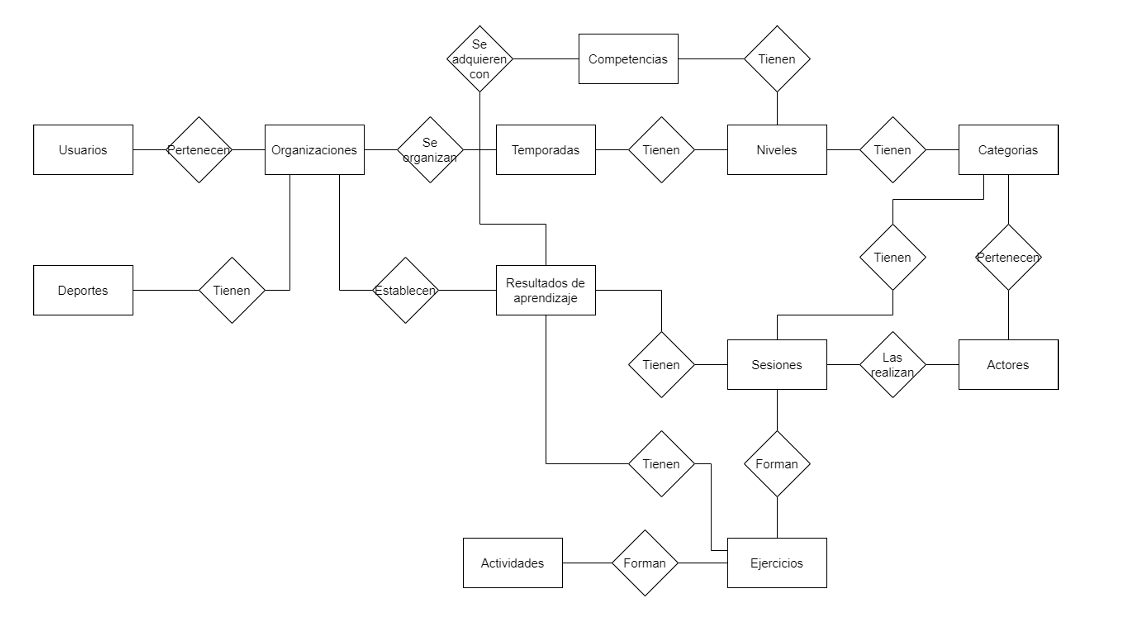
\includegraphics[width=15cm]{archivos/tfg_jorge/esquema_conceptual_Sergio}
    \caption{Mapa conceptual de Sergio Yáñez Cánovas y Daniel Gónzalez Luque}\label{sistemass2}
\end{figure}

Después de analizar el mapa conceptual, con la base de datos que se nos ha proporcionado podemos analizar el modelo Entidad-Relación, donde estarán expresadas las relaciones y atributos entre las entidades de ésta.

\begin{figure}[H]
    \centering
    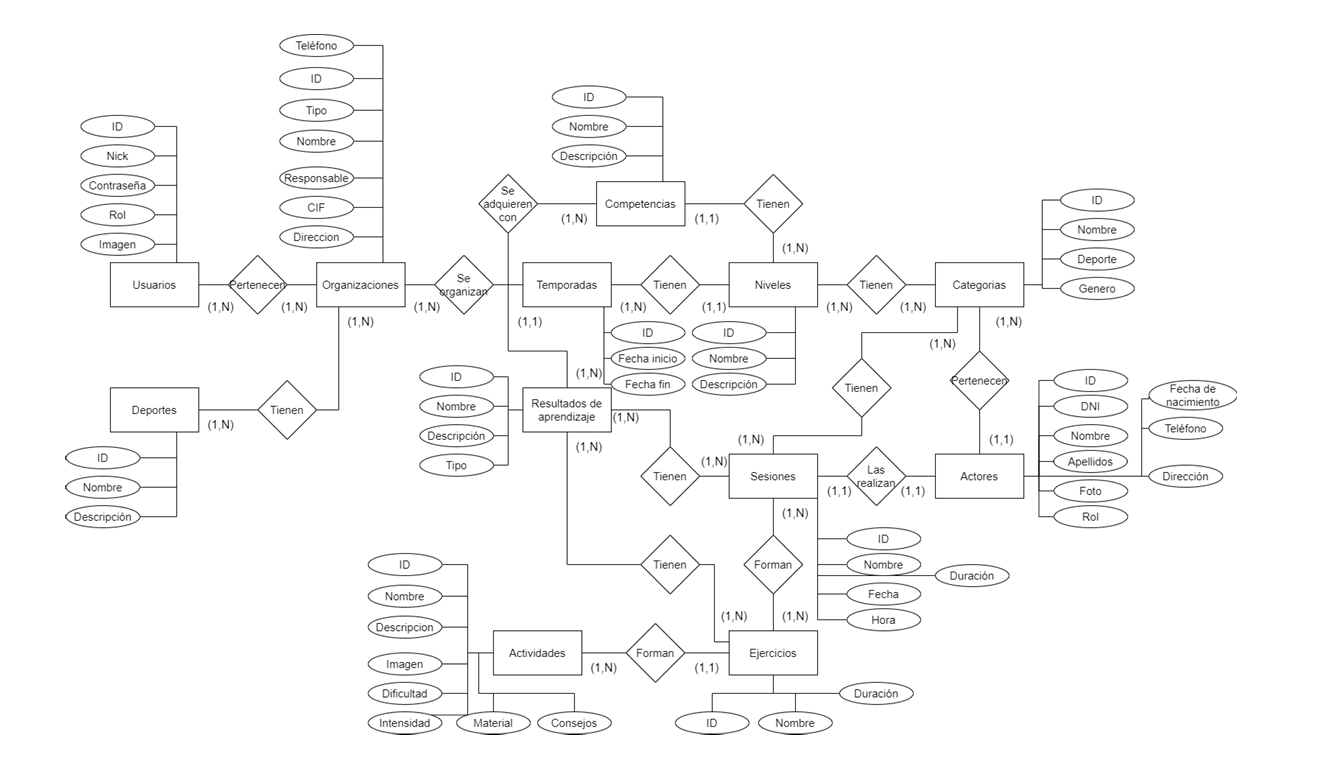
\includegraphics[width=15cm]{archivos/tfg_jorge/esquema_entidad_rel_Sergio}
    \caption{Modelo Entidad-Relación de Sergio Yáñez Cánovas y Daniel Gónzalez Luque}\label{sistemass2}
\end{figure}

\subsection{Análisis de interfaces}
\label{subsec:int_analysis}
En este apartado presentaremos una descripción detallada de las interfaces de usuario. Las interfaces estarán enfocadas pensando en una aplicación accesible por cualquier navegador. Puesto que a Internet pueden acceder tanto ordenadores como dispositivos móviles, debemos asegurarnos de que las interfaces sean \textit{responsive}.
Por otro lado, sabiendo que el análisis puede hacerse desde cualquier sitio, procuraremos que el usuario obtenga la interfaz lo más intuitiva y rápida posible.

\subsubsection{Inicio de sesión}
Esta interfaz permitirá al usuario autenticarse en la aplicación, contendrá los campos para introducir el correo electrónico y la contraseña del usuario.
\subsubsection{Selección de organización}
Esta interfaz obtendrá de la base de datos las organizaciones a las que el usuario iniciado figura como actor. Mostrará las organizaciones en forma de botón para poder ser seleccionadas y pasar a la vista principal.
\subsubsection{Pantalla principal de la organización}
Muestra una visión general de la organización, dentro de esa visión general se incluirá una versión resumida de las diferentes interfaces de la aplicación (Organización, Estadísticas y Calendario). Sobre la organización mostrará una lista con los nombres de los jugadores (Actores en la base de datos de tipo 2).
Sobre las estadísticas mostrará dos cuadros, el primero será un listado de los KPIs calculados de las sesiones individuales de cada jugador y mostrados de manera grupal. El segundo será una pequeña columna de gráficos sobre dichos KPIs.
Por último, en la parte inferior se mostrará un pequeño calendario que mostrará las sesiones extraídas de la base de datos.
\subsubsection{Detalles del Actor}
Presenta información detalla sobre un jugador específico, mostrando la información dividida en cinco cuadros.
El primer cuadro mostrará los datos personales del jugador (foto de perfil, nombre y apellidos, fecha de nacimiento, DNI y teléfono).
El segundo cuadro mostrará los KPIs que ese jugador ha entrenado por lo menos una vez, junto con la evaluación de rendimiento de cada ejercicio.
El tercero contendrá una matriz DAFO (debilidades, amenazas, fortalezas y oportunidades) calculada a partir de un análisis estadístico a partir de las diferentes evaluaciones a lo largo del tiempo.
El cuarto cuadro contendrá los gráficos de la evolución de los KPIs.
Por último, el último cuadro contendrá el historial de partidos del jugador con los minutos jugados.
\subsubsection{Estadísticas}
Proporciona una vista detallada de las estadísticas de la organización a través de gráficos de varios KPIs. Incluirá botones para generar informes de todos los KPIs.
\subsubsection{Calendario}
Permite una navegación sencilla entre las fechas del año para mostrar todas las sesiones que tienen que ver con la organización seleccionada por el usuario.
\subsubsection{Menú}
Será implantado en todas las interfaces, dispondrá de un menú superior y uno lateral.
El menú superior mostrará el nombre de la organización seleccionada, el nombre de la interfaz actual, el nombre y foto del usuario de la sesión junto con un botón de cerrar sesión.
Este menú superior contendrá un menú inferior donde el usuario podrá elegir el intervalo de tiempo de la recogida de KPIs, dicho intervalo se aplicará a todas las interfaces.
El menú lateral será un menú desplegable que contendrá las diferentes vistas de la aplicación, desplegado se verá el nombre junto al icono mientras que si no lo está solo se verá el icono.
\subsection{Análisis de servicios}
Este trabajo seguirá una arquitectura basada en un patrón de diseño MVC (Modelo-Vista-Controlador) implementado con Vue.js. Describiremos los servicios que nuestra aplicación proporcionará, enfocados en la gestión y el análisis de la organización y sus actores.

\subsubsection{Autenticación}
\begin{itemize}
    \item Validar las credenciales del usuario con la base de datos.
    \item Obtener un token de sesión para el framework DAO.
    \item Manejar el cierre de sesión eliminando el token de autenticación.
\end{itemize}
\subsubsection{Organizaciones}
\begin{itemize}
    \item Consultar y devolver las organizaciones asociadas al usuario autenticado.
    \item Establecer la organización seleccionada durante la sesión.
\end{itemize}
\subsubsection{Actores}
\begin{itemize}
    \item Consultar y devolver la lista de actores que pertenecen a la organización seleccionada.
    \item Consultar y devolver la información detallada de un jugador específico, incluyendo datos personales y registros de su rendimiento.
\end{itemize}
\subsubsection{Estadísticas}
\begin{itemize}
    \item Consultar y devolver los KPIs de forma grupal para toda la organización.
    \item Consultar y devolver los KPIs de forma individual de un actor específico de la organización.
    \item Generar una matriz DAFO a partir de un análisis estadístico de los datos obtenidos.
    \item Generar informes en formatos .pdf o .csv de todos los KPIs.
    \item Actualizar las consultas seleccionando el intervalo de tiempo para la visualización de estadísticas y gráficos.
\end{itemize}
\subsubsection{Calendario}
\begin{itemize}
    \item Consultar y devolver las sesiones de la base de datos sobre la organización seleccionada.
    \item Permitir la visualización del calendario en diferentes periodos.
\end{itemize}
\section{Diseño del sistema}
\subsection{Arquitectura general}
Siguiendo los trabajos de [\cite{TFG_Daniel}] y [\cite{TFG_Sergio}], ellos definen que "la estructura de su sistema estará formada por 4 fases: planificación, ejecución, análisis y 
evaluación, que forman un ciclo completo y cíclico para el desarrollo de los deportistas."

\begin{figure}[H]
    \centering
    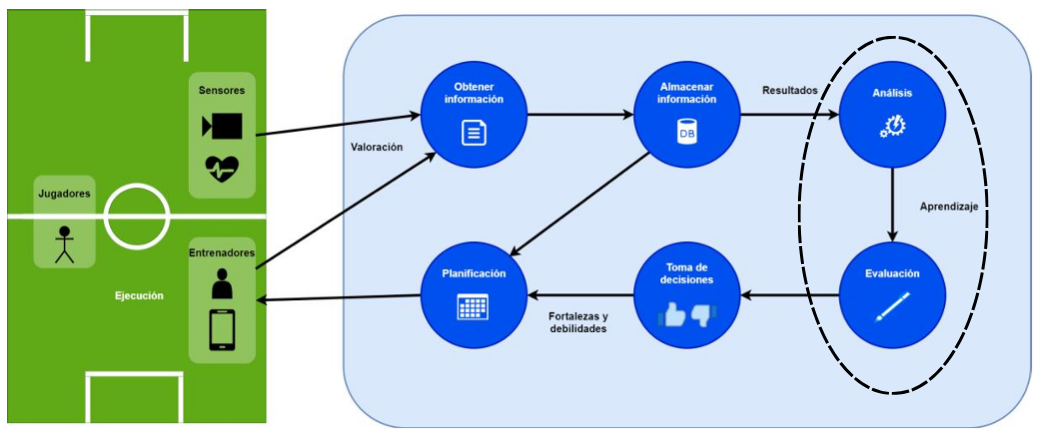
\includegraphics[width=15cm]{archivos/tfg_jorge/arquitectura_general_Sergio}
    \caption{Arquitectura general del sistema de Sergio Yáñez Cánovas y Daniel Gónzalez Luque}\label{sistemass2}
\end{figure}

Nuestro sistema se centrará en la fase de \textbf{análisis y la de evaluación} de los datos recopilados.
Una vez acabe la fase de recopilación y almacenamiento de datos, la información será totalmente visible a través de la aplicación web. Esta información conllevará los nuevos resultados de la sesión dados por el entrenador y la actualización de los gráficos y las matrices DAFO de cada jugador.
Para la actualización de los nuevos resultados de la matriz DAFO, se volverá a hacer el cálculo estadístico siguiendo cada resultado de nuevo teniendo en cuenta que se evalúan las pendientes y la consistencia del jugador. Una vez la aplicación obtenga los resultados serán totalmente visibles para el usuario.
\subsection{Diseño de interfaces de usuario}
A continuación, se mostrarán los mockups elaborados para todas las interfaces definidas en \hyperref[subsec:int_analysis]{Análisis de interfaces}. Estas interfaces pueden ser modificadas a lo largo del trabajo.

\subsubsection{Inicio de sesión}
\begin{figure}[H]
    \centering
    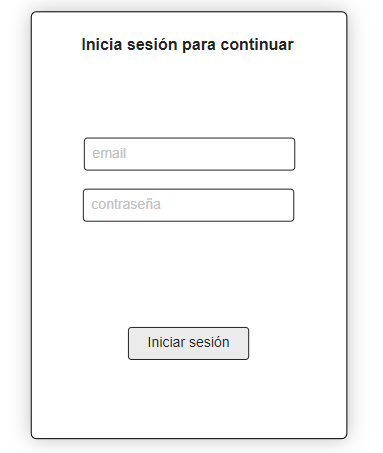
\includegraphics[width=7cm]{archivos/tfg_jorge/mockups/login}
    \caption{Mockup de inicio de sesión}\label{sistemass2}
\end{figure}
Este \textit{mockup} es lo que verá el usuario nada más entre en la aplicación, solo tendrá que introducir el correo electrónico y la contraseña correspondientes para iniciar su sesión.
\subsubsection{Selección de organización}
\begin{figure}[H] 
    \centering
    
\includegraphics[width=8cm]{archivos/tfg_jorge/mockups/seleccion_equipo}
    \caption{Mockup de selección de equipo}\label{sistemass2}
\end{figure}
Una vez iniciada la sesión, el usuario verá las organizaciones que están relacionadas con él, pudiendo seleccionar cualquiera de ellas.
\subsubsection{Página principal}
\begin{figure}[H] 
    \centering
    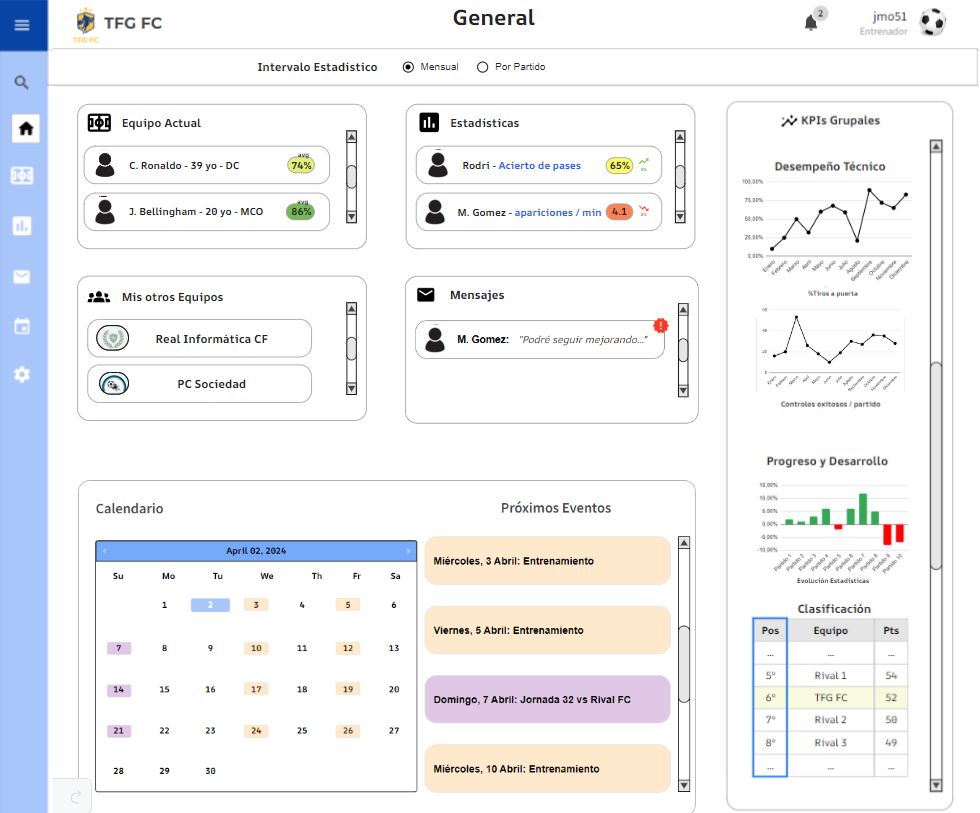
\includegraphics[width=8cm]{archivos/tfg_jorge/mockups/home}
    \caption{Mockup de la página principal}\label{sistemass2}
\end{figure}
Una vez seleccionada la organización, se mostrará una vista principal con las funciones resumidas de la aplicación.
\subsubsection{Equipo}
\begin{figure}[H] 
    \centering
    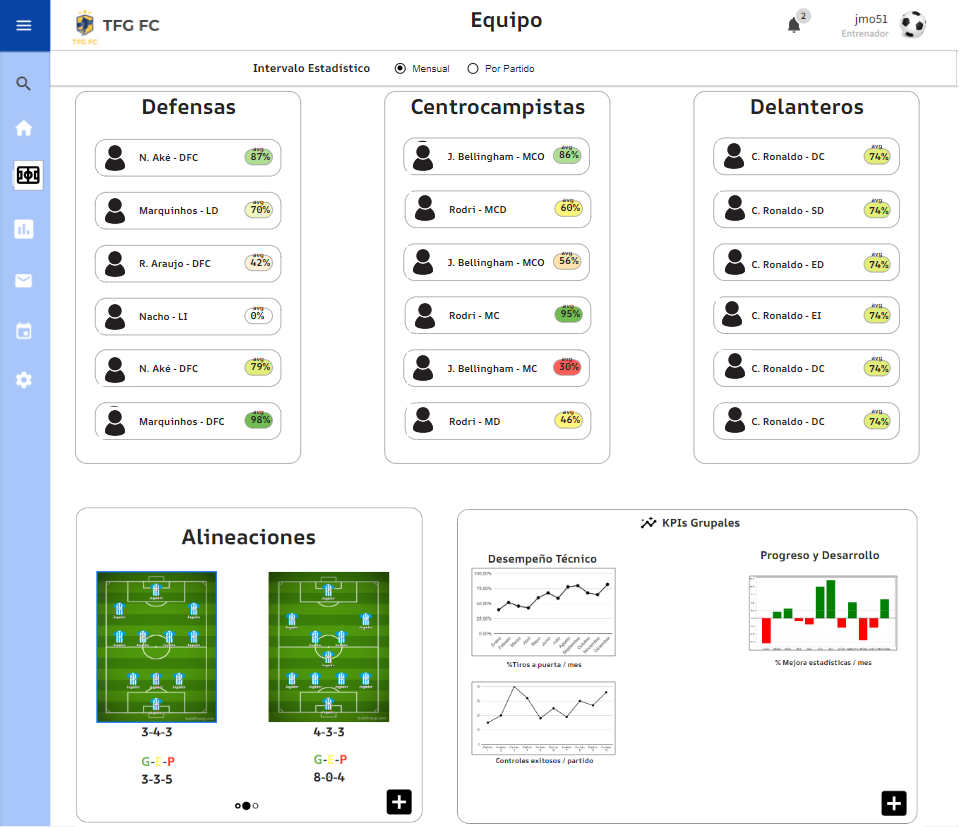
\includegraphics[width=8cm]{archivos/tfg_jorge/mockups/equipo}
    \caption{Mockup de la página de equipo}\label{sistemass2}
\end{figure}
Pudiendo seleccionar esta vista desde la vista principal o desde el menú lateral, mostrará un listado de todos los jugadores que componen la organización, junto con alineaciones que se han dado y sus estadísticas.
\subsubsection{Jugador}
\begin{figure}[H] 
    \centering
    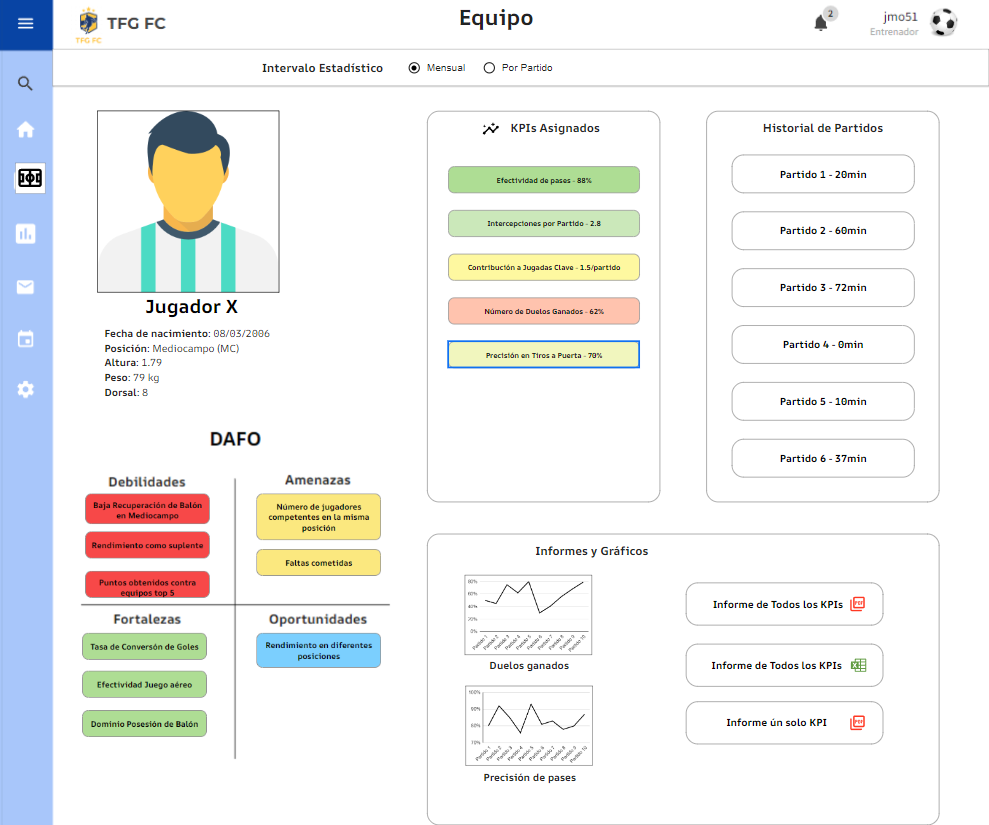
\includegraphics[width=8cm]{archivos/tfg_jorge/mockups/jugador}
    \caption{Mockup de la página de jugador}\label{sistemass2}
\end{figure}
A esta vista se accederá haciendo click sobre un jugador, ya sea en la vista principal o en al vista del equipo. Esta vista mostrará su información personal, su seguimiento de estadísticas y una matriz DAFO para guiar al usuario sobre su rendimiento de una forma más precisa.
\subsubsection{Estadísticas}
\begin{figure}[H] 
    \centering
    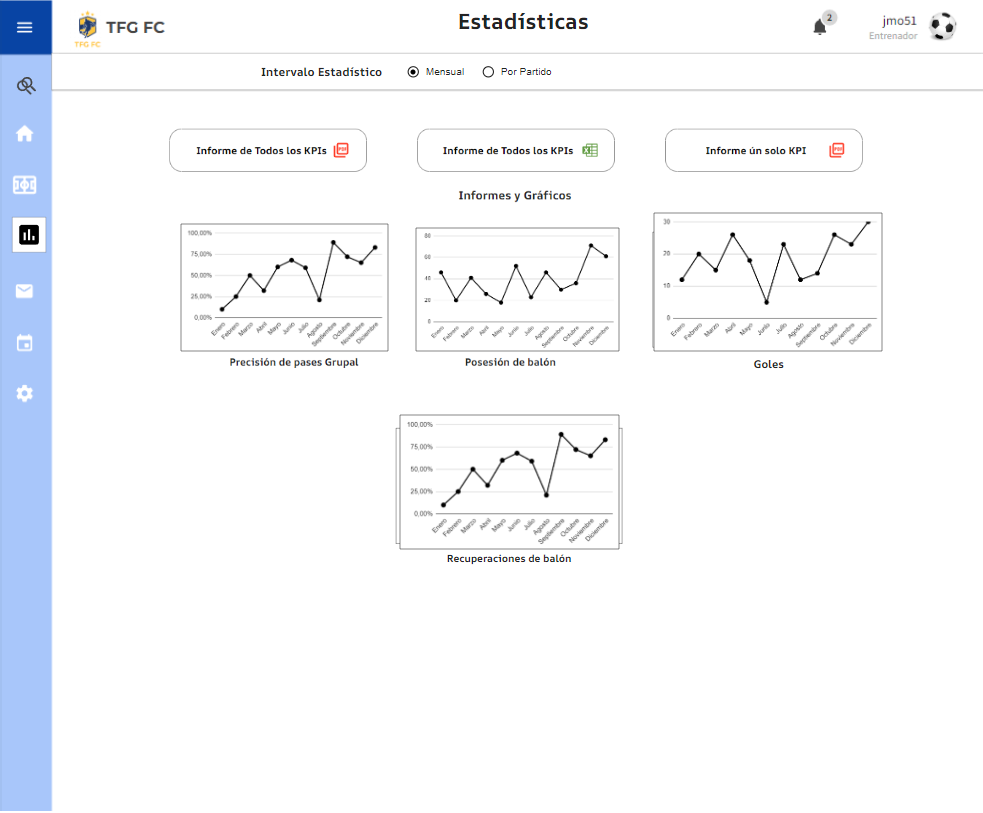
\includegraphics[width=8cm]{archivos/tfg_jorge/mockups/stats}
    \caption{Mockup de la página de estadísticas}\label{sistemass2}
\end{figure}
Pudiendo seleccionar esta vista desde la vista principal o desde el menú lateral, mostrará un listado de gráficos sobre la evolución de las puntuaciones dadas por el entrenador durante las sesiones.
\subsubsection{Calendario}
\begin{figure}[H] 
    \centering
    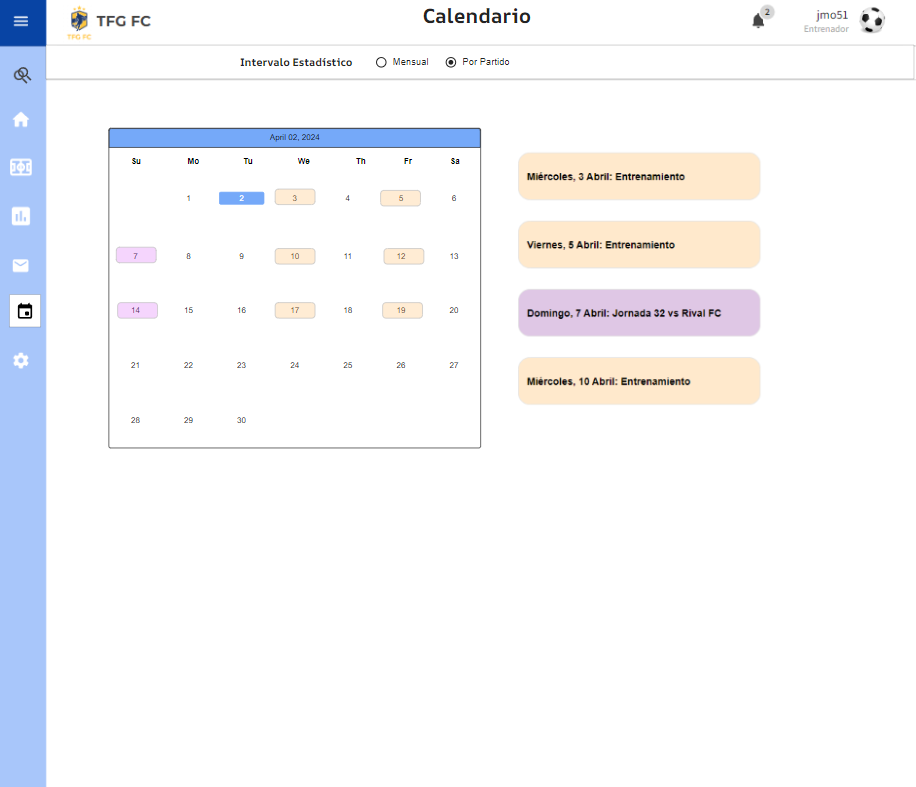
\includegraphics[width=8cm]{archivos/tfg_jorge/mockups/calendario}
    \caption{Mockup de la página de calendario}\label{sistemass2}
\end{figure}
esta vista también será accesible por el menú lateral y por la vista principal. Mostrará un calendario junto con las sesiones más próximas.
\subsection{Diseño lógico de la base de datos}
Dado el apartado de \hyperref[subsec:ent_nego_analysis]{Análisis de entidades de negocio}, el diseño del modelo lógico de la base de datos que vamos a utilizar vendrá dado gracias a los trabajos de [\cite{TFG_Daniel} y [\cite{TFG_Sergio}]:
\begin{figure}[H]
    \centering
    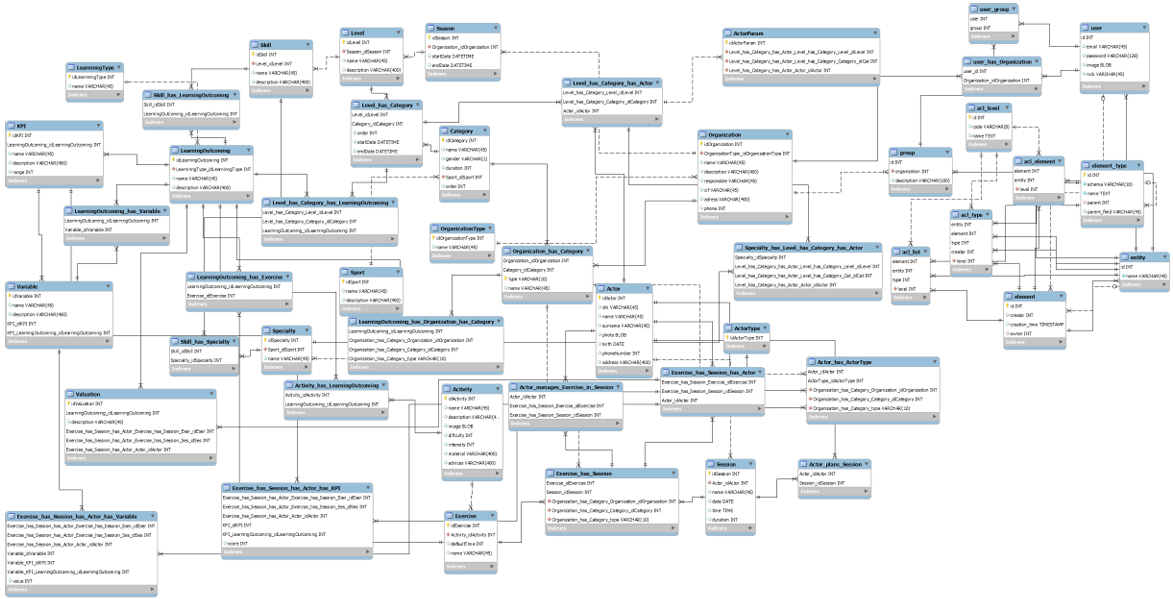
\includegraphics[width=15cm]{archivos/tfg_jorge/logical_design_bbdd}
    \caption{Modelo lógico de Sergio Yáñez Cánovas y Daniel Gónzalez Luque}\label{sistemass2}
\end{figure}
Dado este esquema lógico, procederemos a analizar las principales tablas a las que accederemos durante la implementación del proyecto.
\subsubsection{User}
Esta tabla contiene los atributos: email, nick, password e image. Los atributos email y password se utilizarán para validar el inicio de sesión del usuario, mientras que los atributos nick e image serán utilizados en la cabecera de la aplicación para mostrar al usuario que ha iniciado la sesión.
\subsubsection{Organization}
En esta tabla se almacenan los datos de las organizaciones, de la que solamente accederemos a su ID y su nombre para ser mostrado por pantalla.
\subsubsection{User has organization}
Contiene la información necesaria para saber si el usuario que ha iniciado sesión pertenece a una organización de la base de datos.
\begin{figure}[H]
    \centering
    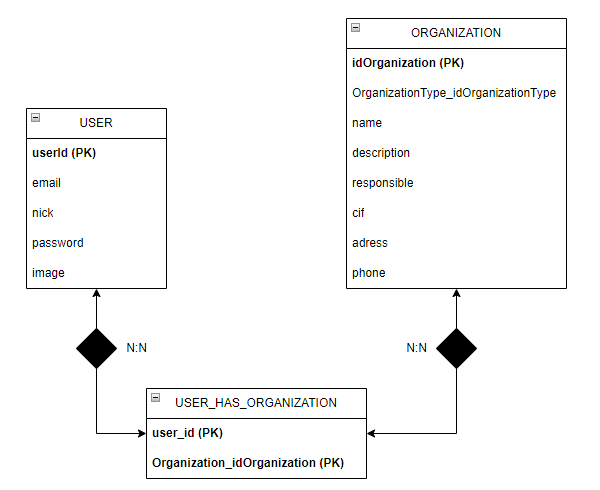
\includegraphics[width=8cm]{archivos/tfg_jorge/modelo_logico/rel_user_org}
    \caption{Relación entre las tablas user, organization y user has organization}\label{sistemass2}
\end{figure}
\subsubsection{Actor}
Contiene la información de los actores que componen la organización, como se define en los trabajos de Sergio y Daniel: "Un actor es cualquier participante o miembro de la organización. Jugadores, Entrenadores, Preparadores físicos, Entrenadores de porteros, Coordinadores, ..." [\cite{TFG_Daniel}, [\cite{TFG_Sergio}]. Esta tabla será utilizada para extraer la información personal de cada jugador, así como verificar las sesiones asociadas con dicha organización.
\subsubsection{Session}
Almacena los datos de las sesiones de la organización (nombre, fecha, hora y duración) llevadas por un actor. Estos datos serán extraídos para rellenar el calendario de la aplicación y también para analizar los resultados de sesiones pasadas.
\subsubsection{Actor has actortype}
Indica el tipo de actor dentro de una organización dada, analizando los datos de la base de datos, podemos concluir que el tipo actor '2' corresponde a los jugadores, mientras que el tipo actor '1' a los entrenadores o coordinadores de la organización. Esta información la utilizaremos para extraer a todos los actores de tipo '2' (Jugadores) para hacer un listado en la aplicación.
\subsubsection{Kpi}
Se utiliza para almacenar los indicadores clave de rendimiento (Key Performance Indicators), están relacionados con resultados de aprendizaje 'Learning Outcomes'. Los usaremos para extraer su nombre para relacionarlo con la puntuación de cada ejercicio.
\subsubsection{Exercise}
Servirá para obtener el nombre del ejercicio que se ha realizado para mostrarlo en el análisis. Como se define en los trabajos de [\cite{TFG_Daniel} y [\cite{TFG_Sergio}]: "Un ejercicio es una actividad concreta con una duración de tiempo y que deberá ser realizado por un equipo o un conjunto de actores.Un ejercicio es definido para entrenar uno o varios resultados de aprendizajes y debe indicarse si es para todo el equipo, si es un deporte de equipo, o para miembros concretos. Se debe indicar el orden de los ejercicios en la sesión, que lo indicará la posición en la IU. Un ejercicio debe tener un duración concreta."
\subsubsection{Exercise has session has actor has kpi}
De esta tabla obtendremos la puntuación de los ejercicios realizados por un actor dentro de una sesión dada. La puntuación de los ejercicios estará ligada a un KPI de la base de datos, información que será mostrada en el análisis del equipo y de cada jugador.

\begin{figure}[H]
    \centering
    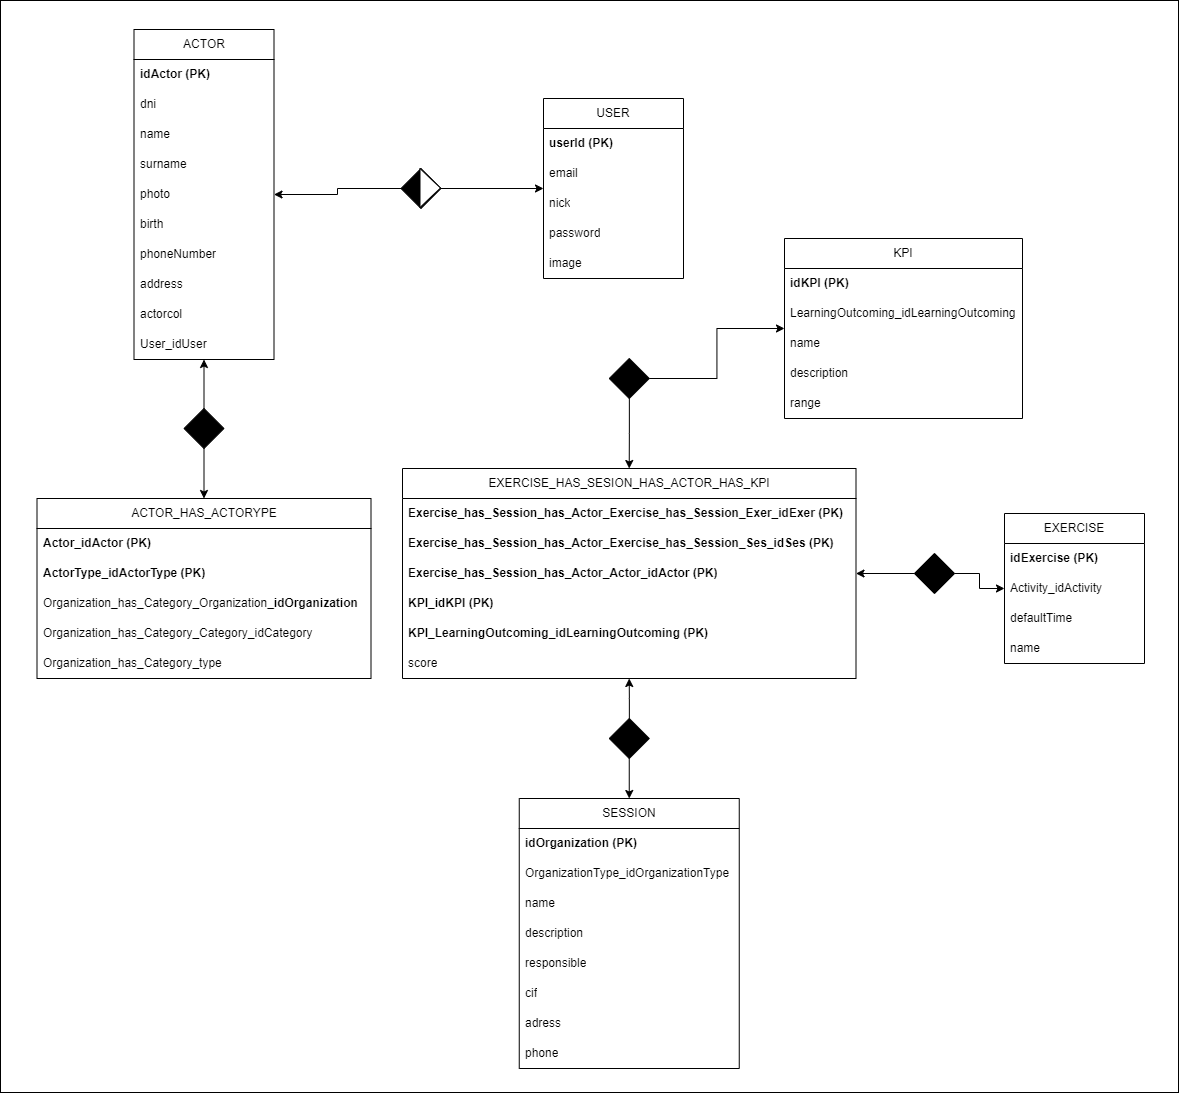
\includegraphics[width=8cm]{archivos/tfg_jorge/modelo_logico/exercises_kpi}
    \caption{Relación entre las tablas user, actor, session, actor has actortype, kpi, exercise, exercise has session has actor has kpi}\label{sistemass2}
\end{figure}
\subsection{Diseño de servicios}
A continuación explicaremos el diseño de los servicios mencionados anteriormente. Se habrá diseñado una API REST basada en HTTP, dicha API es bastante simple y ha sido proporcionada por [\cite{TFG_Daniel}], [\cite{TFG_Sergio}] y mis tutores Virgilio Gilart Iglesias y Diego Marcos Jorquera.
La API define operaciones CRUD básicas, en nuestro caso, solo serán necesarias las operaciones GET sobre cualquier entidad Foo:
\begin{itemize}
\item GET/api/v1/foos
\item GET/api/v1/foos/id
\end{itemize}
Los tipos de datos estarán escritos en formato JSON, a continuación mostraremos los tipos de datos de los esquemas que hemos utilizado:
\begin{lstlisting}[style=Consola, caption={Tipo dato user},label=Consola_code_user]
user: 
	type: object 
   	displayName: User 
   	description: Usuario de una organización 
   	properties: 
     	image: blob 
     	userId: string 
     	email: string 
    	nick: string 
     	password: password 
     	aclElement: aclElement[] 
     	aclType: aclType[] 
     	aclList: aclList[] 
     	groups: userGroup[] 
\end{lstlisting}
\begin{lstlisting}[style=Consola, caption={Tipo dato organización},label=Consola_code_org]
organization:
	type: object
 	displayName: Organization
 	description: Organization
 	properties
 		idOrganization:integer
		OrganizationType_idOrganizationType:int
		name:string
		description:string
		responsible:string
		cif:string
		adress:string
		phone:string
\end{lstlisting}
\begin{lstlisting}[style=Consola, caption={Tipo dato actor},label=Consola_code_actor]
actor: 
	type: object 
	displayName: actor 
	description: Información de un actor 
	properties: 
		idActor: integer 
		dni: string 
		name: string 
		surname: string 
		photo: blob 
		birth: datetime 
		phoneNumber: int 
		address: string
\end{lstlisting}
\begin{lstlisting}[style=Consola, caption={Tipo dato sesión},label=Consola_code_sesion]
session: 
   	type: object 
    displayName: session
    description: Sesiones de una organización 
    properties: 
    	idSession: integer 
      	Actor_idActor: int 
      	name: string 
      	date: datetime 
      	time: time 
      	duration: int
\end{lstlisting}
\begin{lstlisting}[style=Consola, caption={Tipo dato kpi},label=Consola_code_kpi]
kpi:
	type: object
 	displayName: KPI
 	description: KPIs de un resultado de aprendizaje
 	properties
 		idKPI: integer
 		LearningOutcoming_idLearningOutcoming: int
 		name: string
 		description:string
 		range:int
\end{lstlisting}
\begin{lstlisting}[style=Consola, caption={Tipo dato exercise},label=Consola_code_exercise]
exercise: 
    type: object 
    displayName: exercise 
    description: Ejercicios de una sesión de entrenamiento 
    properties: 
      	idExercise: integer 
      	Activity_idActivity: int 
      	defaultTime: int 
      	name: string
\end{lstlisting}

Con esta API y los tipos de datos, seremos capaz de implementar las pertinentes consultar GET para después elaborar la lógica en el lado del cliente y mostrar los resultados.
\section{Implementación}
\subsection{Arquitectura técnica}
Explicaremos como funciona la arquitectura de la aplicación de Vue.js, que funciona conjuntamente con el lado del servidor que nos ha sido proporcionado.

\begin{figure}[H]
    \centering
    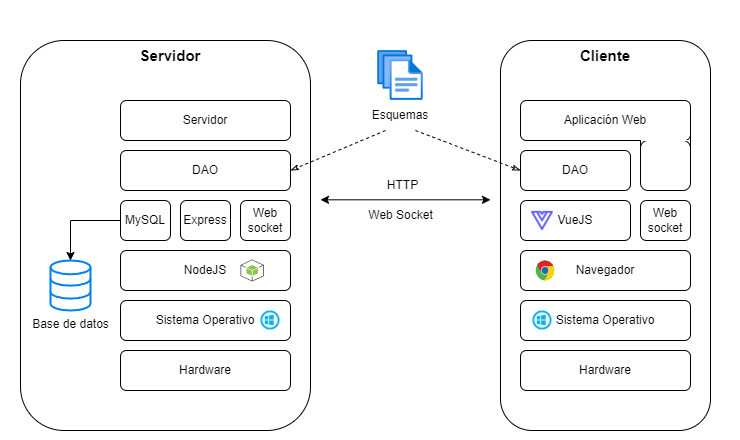
\includegraphics[width=15cm]{archivos/tfg_jorge/arquitectura_tecnica}
    \caption{Arquitectura técnica del sistema}\label{sistemass2}
\end{figure}

Tanto en el cliente como en el servidor, las dos capas inferiores corresponderán al hardware y al sistema operativo sobre el que se despliegue la aplicación, en mi caso, la aplicación de Vue ha sido desarrollada en Windows 10.

Siguiendo por el lado del servidor desarrollado en [\cite{TFG_Daniel}] y [\cite{TFG_Sergio}], la siguiente capa será conformada por el framework de servidor Node.js, que será el encargado de procesar las peticiones y generar las respuestas hacia el cliente.

La siguiente capa la conforman la aplicación que administra la base de datos de la aplicación, MySQL, Express será utilizado como framework de Node para la creación de los servicios. Y por último WebSocket [\cite{def_websocket}], que realiza las conexiones cliente-servidor.

En la siguiente capa superior estará el framework DAO (Data Access Object) proporcionado por nuestro tutor. Se trata de un framework que gestiona los accesos a la base de datos, haciendo las peticiones desde la aplicación de Vue.js mucho mas sencillas.

En la capa superior se encuentra la lógica del servidor, que puede incluye lógica de negocio y controladores que orquestan las diferentes partes de la aplicación.

Siguiendo por el lado del Cliente, posterior a las capas de hardware y sistema operativo, se encuentra la capa del navegador, que permite a los usuarios interactuar con la aplicación web.

La siguiente capa la conforman WebSocket, utilizado para mantener la comunicación en tiempo real con el servidor, y Vue.js, siendo un framework de JavaScript utilizado para construir interfaces de usuario interactivas. [\cite{def_vue}].

En las últimas capas se encontrarán el DAO, contenido dentro de la aplicación web para realizar las peticiones pertinentes. La aplicación web es la interfaz con la que interactúan los usuarios.

\subsection{Implementación de interfaces de usuario}
Mostraremos las interfaces de usuario que hemos desarrollado con Vue.js, los datos que se verán por pantalla son datos inventados de ejemplo para poder realizar la captura de pantalla.

\subsubsection{Inicio de sesión}
\begin{figure}[H]
    \centering
    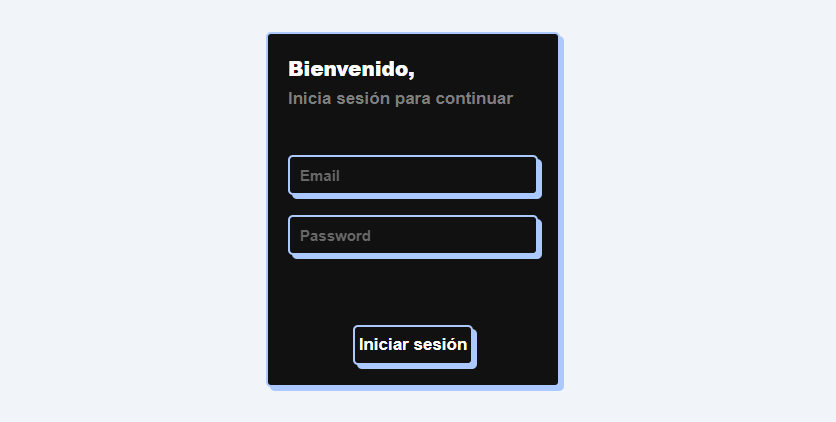
\includegraphics[width=10cm]{archivos/tfg_jorge/interfaces/login}
    \caption{Implentación de la interfaz de inicio de sesión}\label{sistemass2}
\end{figure}

La implementación de esta interfaz ha sido muy similar a la del \textit{mockup}, siendo un cuadro en el que se solicitan el email y la contraseña al usuario.
\subsubsection{Selección de organización}
\begin{figure}[H]
    \centering
    
\includegraphics[width=7cm]{archivos/tfg_jorge/interfaces/seleccion_equipo}
    \caption{Implentación de la interfaz de selección de organización}\label{sistemass2}
\end{figure}

La implementación de esta interfaz también es similar al \textit{mockup}, mostrando las organizaciones que están relacionadas con el usuario iniciado.
\subsubsection{Página principal}
\begin{figure}[H]
    \centering
    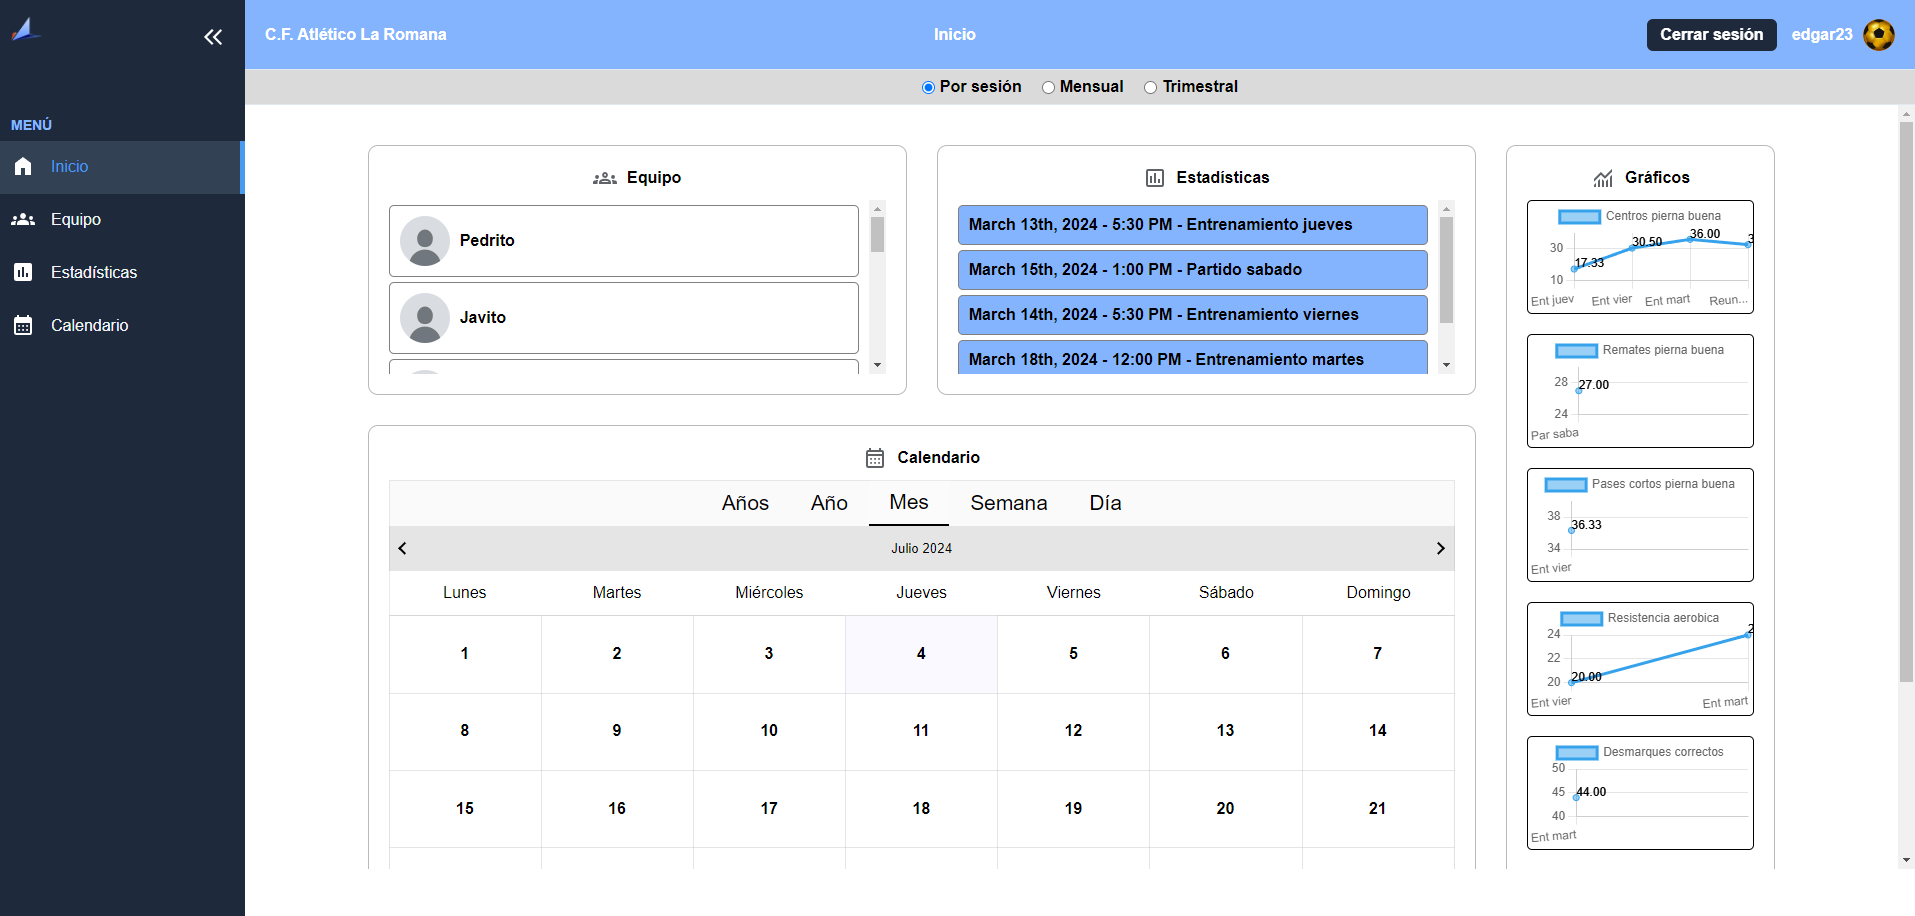
\includegraphics[width=10cm]{archivos/tfg_jorge/interfaces/home}
    \caption{Implentación de la interfaz de la página principal}\label{sistemass2}
\end{figure}

A diferencia del diseño de la interfaz, se han eliminado los cuadros de mis otros equipos, ya que las tablas de la base de datos no admiten que un actor sea entrenador de dos equipos distintos, por lo tanto aunque se implemente en el futuro dejar un cuadro vacío no tendría sentido.

También se ha eliminado el cuadro de mensajes, considerando que la forma de comunicación idónea puede ser durante las sesiones. En la columna de estadísticas se ha eliminado la clasificación, ya que no tenemos acceso a ella, y finalmente los próximos eventos el cuadro del calendario, para no restarle relevancia a la vista completa.
\subsubsection{Equipo}
\begin{figure}[H]
    \centering
    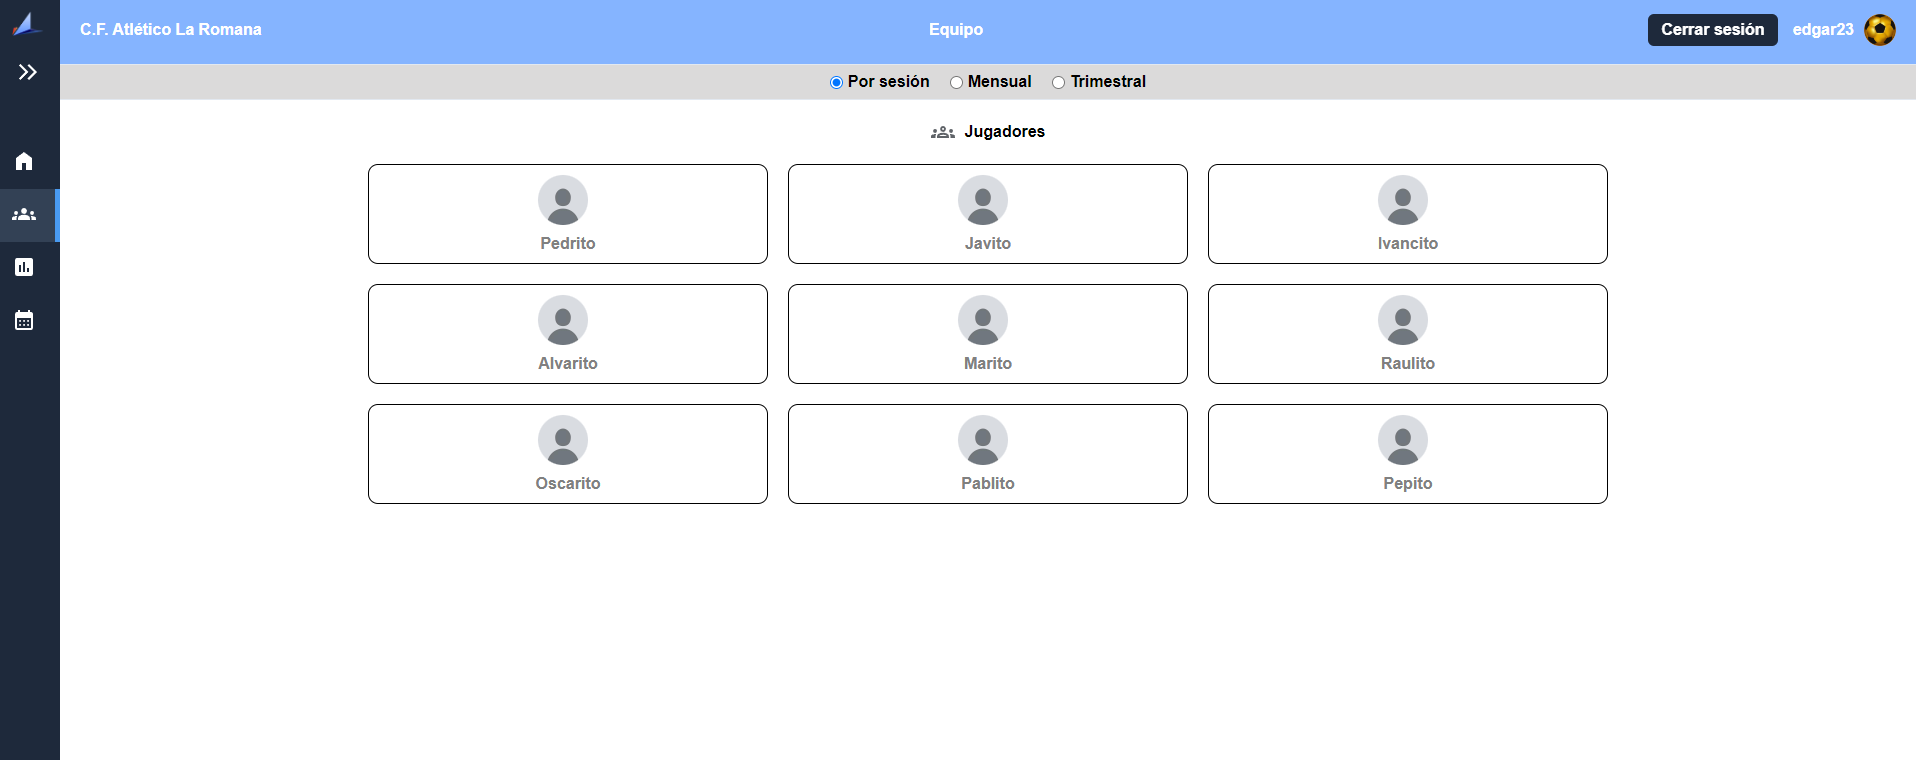
\includegraphics[width=10cm]{archivos/tfg_jorge/interfaces/equipo}
    \caption{Implentación de la interfaz de equipo}\label{sistemass2}
\end{figure}

Esta interfaz puede ser la que más cambios haya recibido. En primer lugar, no se separan jugadores por posiciones. Este dado además de no existir en la base de datos, no es un dato muy recurrente en categorías inferiores de fútbol base.

Tampoco tenemos acceso a las alineaciones que se ha ido utilizando, por lo que descartaremos esa parte. Por último, los gráficos se han eliminado para no restarle importancia al cuadro de las estadísticas.
\subsubsection{Jugador}
\begin{figure}[H]
    \centering
    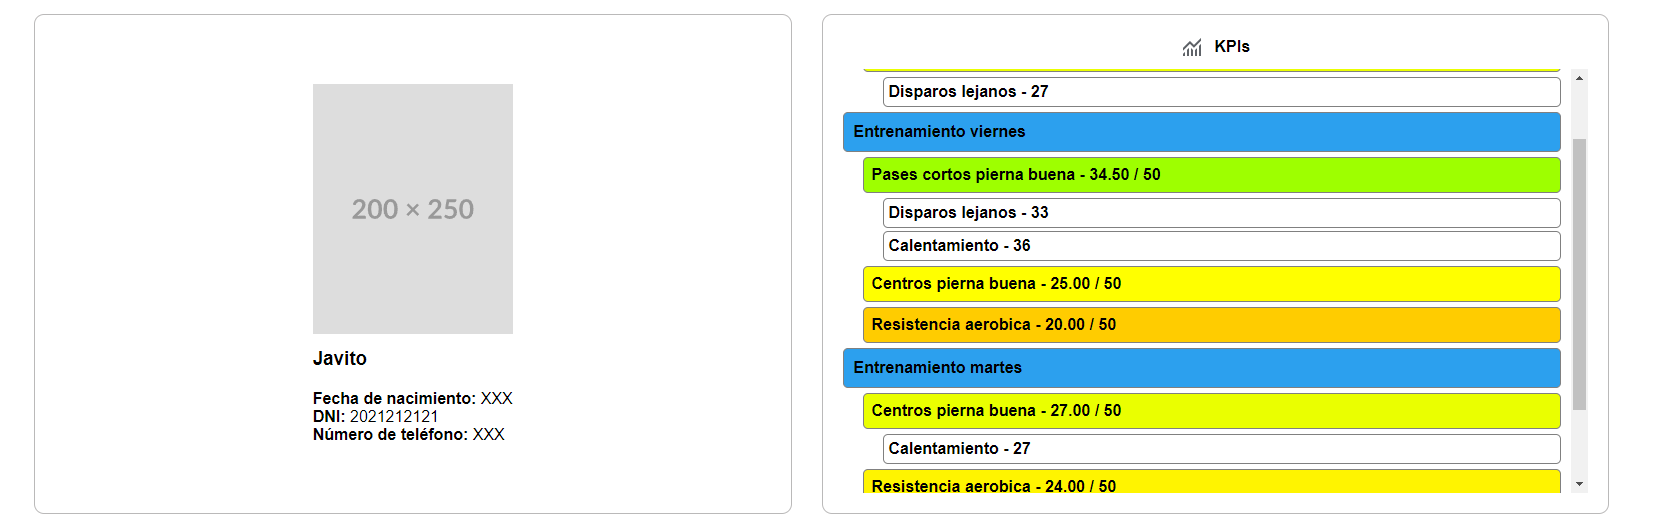
\includegraphics[width=10cm]{archivos/tfg_jorge/interfaces/jugador_1}
    \caption{Implentación de la interfaz de un único jugador - Datos y sesiones}\label{sistemass2}
\end{figure}

\begin{figure}[H]
    \centering
    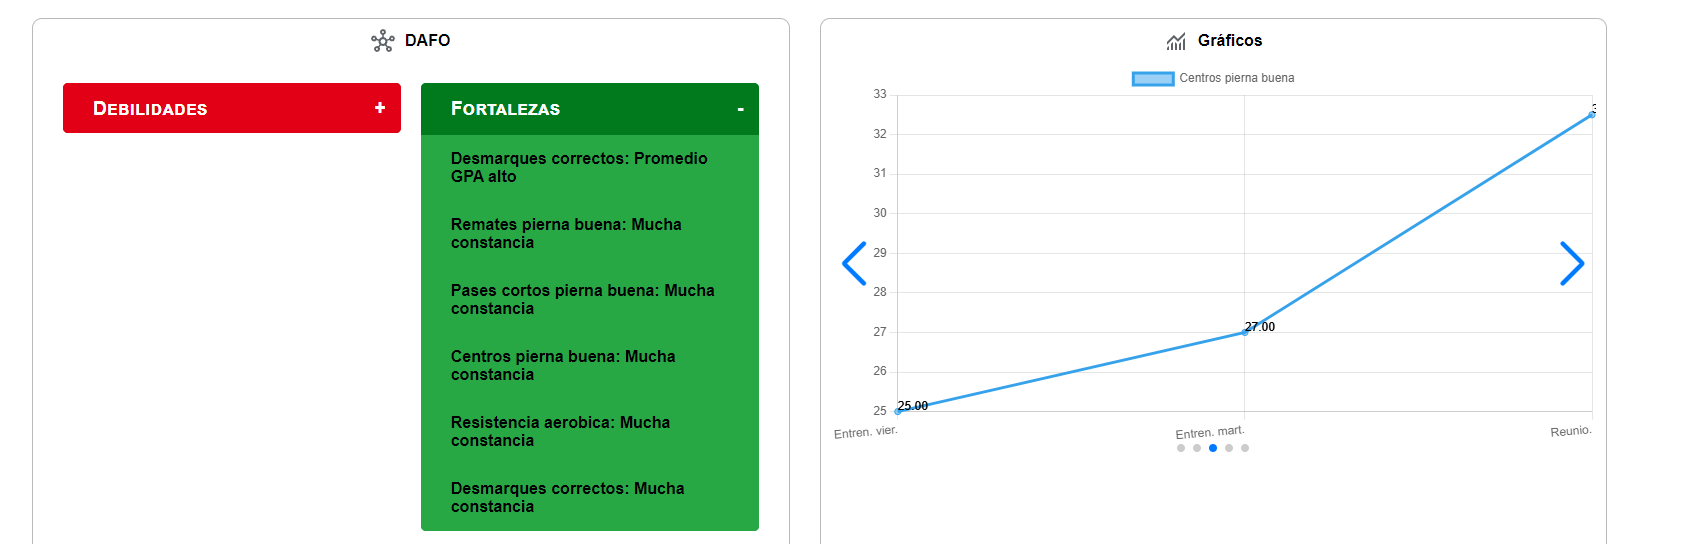
\includegraphics[width=10cm]{archivos/tfg_jorge/interfaces/jugador_2}
    \caption{Implentación de la interfaz de un único jugador - DAFO y gráficos}\label{sistemass2}
\end{figure}

Este diseño también ha sufrido cambios, ahora solo mostrará gráficos en su cuadro correspondiente, para una mayor visibilidad en caso de muchos datos. Adicionalmente, ya no verá el historial de partidos, dado que es un dato del que no disponemos.

La matriz DAFO estará compuesta de las cuatro tarjetas desplegables para la visualización de los datos de una manera más cómoda. También el cuadro antiguo de KPIs asignados ha sido sustituido por un historial de sesiones, meses o trimestres, según lo que indique el menú, de KPIs con sus puntuaciones y ejercicios.
\subsubsection{Estadísticas}
\begin{figure}[H]
    \centering
    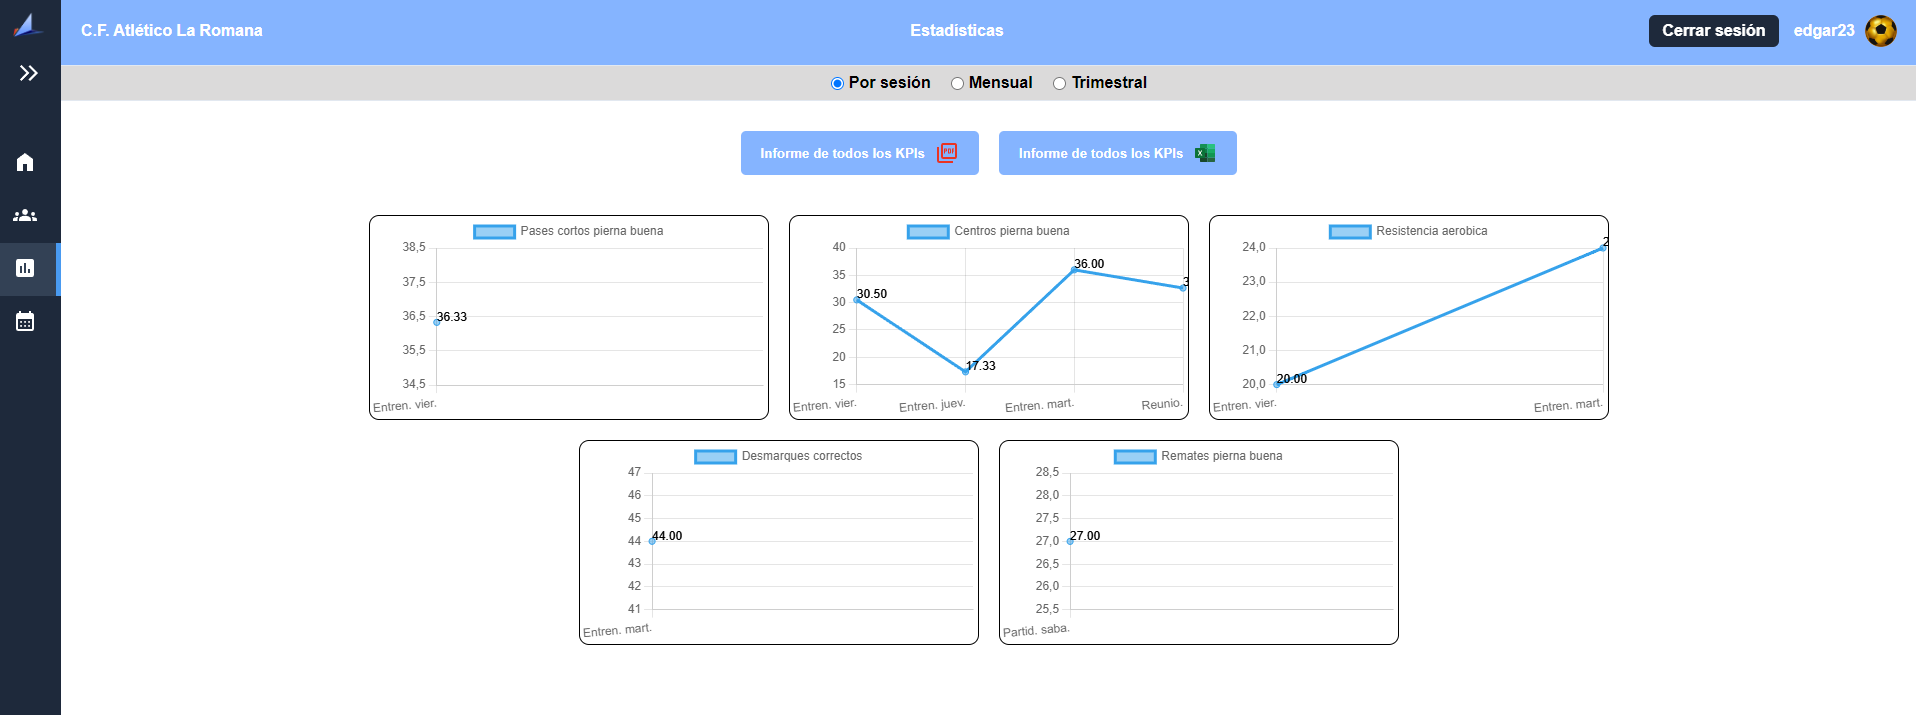
\includegraphics[width=10cm]{archivos/tfg_jorge/interfaces/stats}
    \caption{Implentación de la interfaz de estadísticas}\label{sistemass2}
\end{figure}

Esta vista no ha sufrido muchos cambios comparado con el diseño, teniendo en cuenta que el proyecto trata de leer y analizar datos, ya no se pueden añadir gráficos y KPIs.
\subsubsection{Calendario}
\begin{figure}[H]
    \centering
    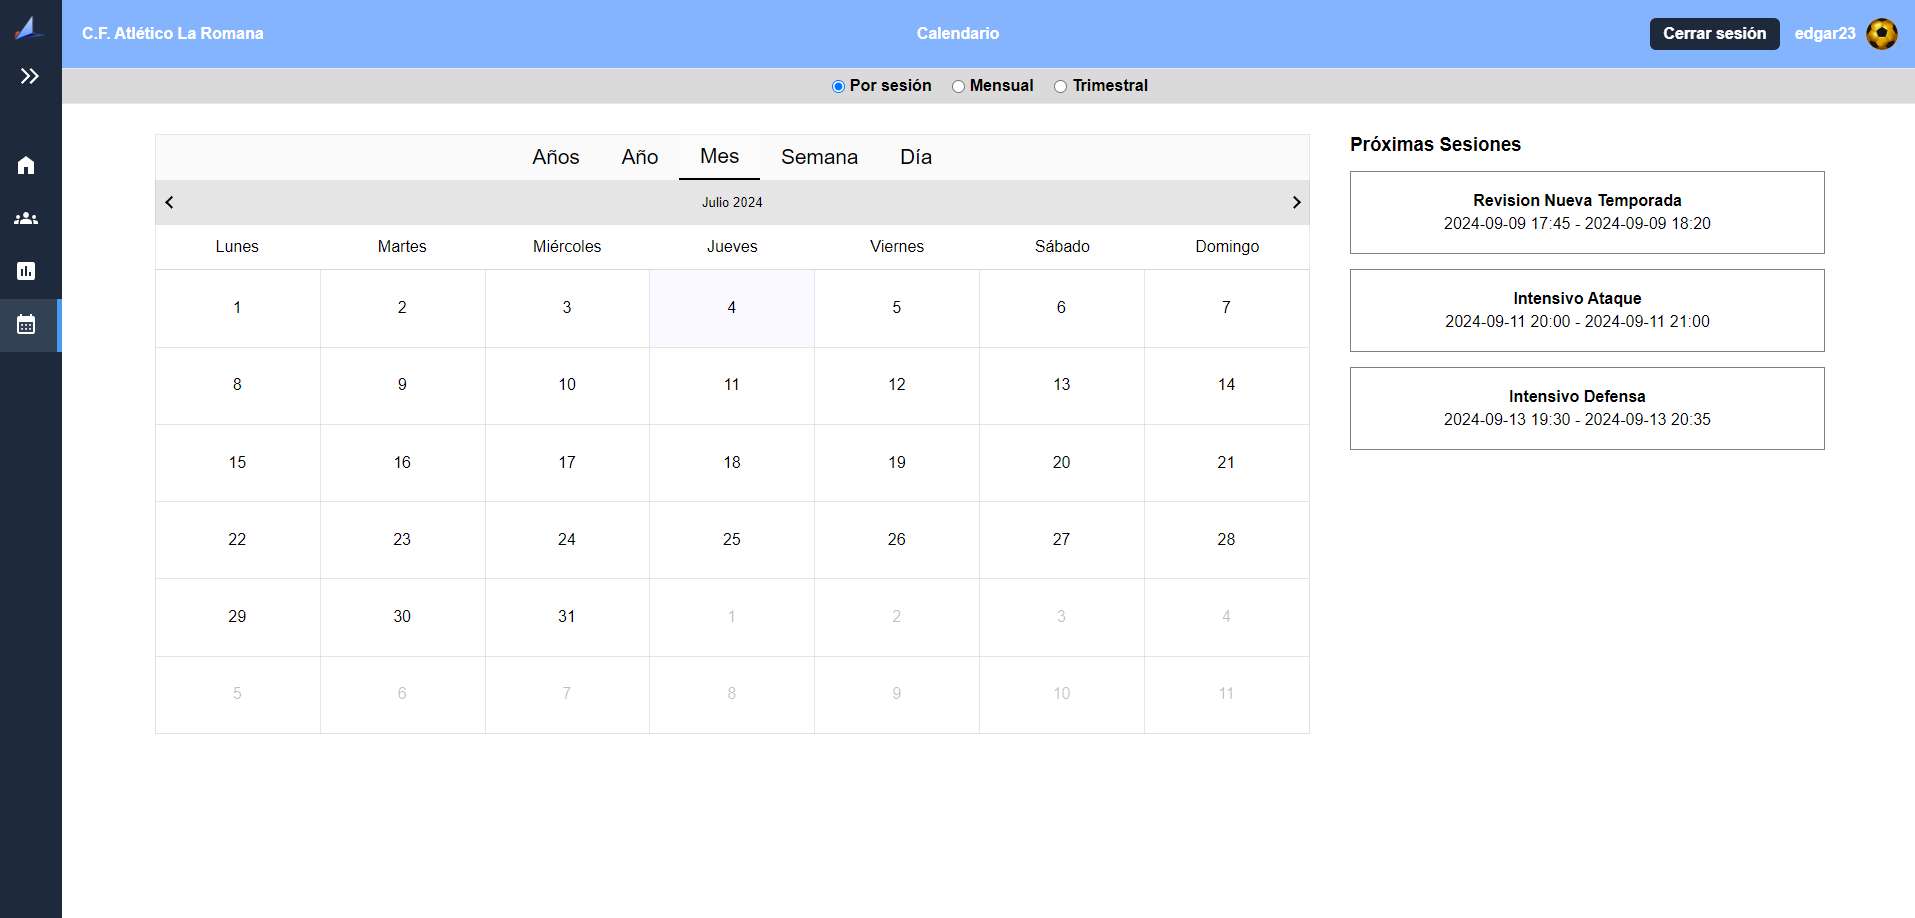
\includegraphics[width=10cm]{archivos/tfg_jorge/interfaces/calendario}
    \caption{Implentación de la interfaz de calendario}\label{sistemass2}
\end{figure}

Esta vista tampoco a sufrido cambios, se muestra el calendario junto con las próximas sesiones que van a acontecer.
\subsection{Esquema físico de la base de datos}
Para mostrar el esquema físico diseñado en los trabajos [\cite{TFG_Daniel}] y [\cite{TFG_Sergio}], se nos ha proporcionado una serie de \textit{scripts} para construir dicho esquema. Ejecutando los \textit{scripts} con el servicio MySQL Server y un \textit{script} para Windows 10, conseguiremos crear el esquema físico de la base de datos.
A continuación mostraré un ejemplo de los \textit{scripts} de la tabla KPI y adicionalmente el \textit{script} utilizado para ejecutarlos.

\begin{lstlisting}[style=Consola, caption={Script para crear la tabla kpi},label=Consola_code_ script_kpi]
CREATE TABLE `kpi` (
	`idKPI` int NOT NULL AUTO_INCREMENT,
  	`LearningOutcoming_idLearningOutcoming` int NOT NULL,
  	`name` varchar(45) DEFAULT NULL,
  	`description` varchar(45) DEFAULT NULL,
  	`range` int DEFAULT NULL,
  	PRIMARY KEY (`idKPI`,`LearningOutcoming_idLearningOutcoming`),
  	KEY `fk_KPI_LearningOutcoming1_idx` (`LearningOutcoming_idLearningOutcoming`),
  	CONSTRAINT `fk_KPI_LearningOutcoming1` FOREIGN KEY (`LearningOutcoming_idLearningOutcoming`) REFERENCES `learningoutcoming` (`idLearningOutcoming`) ON DELETE CASCADE ON UPDATE CASCADE
) ENGINE=InnoDB AUTO_INCREMENT=19 DEFAULT CHARSET=utf8mb3;
\end{lstlisting}

\begin{lstlisting}[style=Consola, caption={Script ejecutar todos los scripts},label=Consola_code_ script_windows]
@echo off

:: Credenciales
set USER=root
set PASSWORD=root
set DATABASE=tfg

:: Directorio donde están los archivos .sql
set DIR=C:\Users\Jorge\Documents\Github Repos\TFG\DB

:: Recorre todos los archivos .sql en el directorio y los importa
for %%f in (%DIR%\*.sql) do (
    mysql -u %USER% -p%PASSWORD% %DATABASE% < %%f
)

echo Importación completada.
pause
\end{lstlisting}

\subsection{Implementación de servicios}
Teniendo los servicios de la API implementados [\cite{TFG_Sergio}][\cite{TFG_Daniel}], podemos proceder a implementar la lógica de nuestros servicios en el lado del cliente.

\subsubsection{Autenticación}
\begin{lstlisting}[style=Javascript-color, caption={Lógica de inicio de sesión en el cliente}, label=Javascript-color_code_auth]
const login = () => {
  app.login({ email: email.value, password: password.value }).then(
    () => {
      dao.user.read().then((response) => {
        let usuario = response.filter(user =>
          user.email == email.value &&
          user.password == password.value
        )[0];

        if(usuario){
          store.dispatch('actualizarLogged', true);
          store.dispatch('actualizarUserID', usuario.id);
          store.dispatch('actualizarUserName', usuario.nick);
        }
        else{
          Swal.fire({
            icon: 'error',
            title: 'Error',
            text: 'Usuario no encontrado',
          });
        }
      }).catch((error) => {
        console.error('Error leyendo los usuarios:', error);
        Swal.fire({
          icon: 'error',
          title: 'Error',
          text: 'Error leyendo los usuarios',
        });
      });
    },
    () => {
      Swal.fire({
        icon: 'error',
        title: 'Error',
        text: 'Error en el login',
      });
    }
  );
};
\end{lstlisting}

\begin{lstlisting}[style=Javascript-color, caption={Lógica de cierre de sesión en el cliente}, label=Javascript-color_code_auth_logout]
logout(){
	this.actualizarLogged(false);
	this.actualizarTeamSelectedID(null);
}
\end{lstlisting}

Con estas funciones, lo primero que haremos será establecer una conexión con el servidor a través de websocket y su función \textit{login(credentials)}. Una vez iniciado sesión en el servidor,podremos verificar las credenciales del usuario en el lado del cliente.

Para el cierre de sesión, modificaremos las variables de entorno pertinentes para que se muestre de nuevo la pantalla de inicio de sesión.

\subsubsection{Organizaciones}
\begin{lstlisting}[style=Javascript-color, caption={Lógica de la obtención de organizaciones},label=Javascript-color_code_selec_team]
cargarOrgs() {
  this.dao.organization.read().then((response) => {
    this.equipos = response.filter(fila => fila.idOrganization == this.user.Organization_idOrganization);
  }).catch(error => {
    console.error('Error al cargar organizaciones:', error);
  });
},
cargarEquipos() {
  this.dao.user_has_organization.read().then((response) => {
    this.user = response.filter(fila => fila.user_id == this.userID)[0];
    this.cargarOrgs();
  }).catch(error => {
    console.error('Error al cargar organizaciones:', error);
  });
},
\end{lstlisting}

Con el usuario iniciado, esta función filtrará las organizaciones relacionadas con él, mostrándolas en pantalla para seleccionarlas.
\subsubsection{Actores}
\begin{lstlisting}[style=Javascript-color, caption={Carga del listado de actores de tipo 2},label=Javascript-color_code_list_players]
async cargarJugadores() {
	if (!this.teamSelectedID) {
		console.error('No team selected');
		return;
	}

	try {
		const response = await this.dao.actor_has_actortype.read();
		this.actores = response.filter(actor =>
			actor.ActorType_idActorType === 2 &&
			actor.Organization_has_Category_Organization_idOrganization === this.teamSelectedID
		);
		this.actorIds = this.actores.map(actor => actor.Actor_idActor);
		await this.cargarDatosCompletosJugadores();
	} catch (error) {
		console.error('Error al cargar jugadores:', error);
	}
},
async cargarDatosCompletosJugadores() {
	try {
		const promises = this.actorIds.map(id => this.dao.actor.read({ idActor: id }));
		this.actoresCompletos = await Promise.all(promises);
		console.log('Datos completos de los actores:', this.actoresCompletos);
	} catch (error) {
		console.error('Error al cargar jugadores completos:', error);
	}
}
\end{lstlisting}

Estas funciones se encargarán de obtener de la base de datos la información de los actores de tipo '2', para posteriormente ser mostrada por pantalla. El uso de \textit{async} y \textit{await} es crucial para manejar operaciones asíncronas de manera estructurada, he decidido implementarlo de esta forma para evitar la carga de datos que no existan y evitar errores innecesarios.

Para cargar la información de un jugador individualmente, solo tenemos que modificar la consulta de los jugadores:

\begin{lstlisting}[style=Javascript-color, caption={Carga de la información de ún solo actor},label=Javascript-color_code_list_singlplayers]
async getPlayerInfo() {
  try {
    const response = await this.dao.actor.read();
    this.informacion_jugador = response.find(actor => actor.idActor == this.$route.query.idActor);
    
    if (this.informacion_jugador) {
      console.log('Info Jugador: ', this.informacion_jugador.idActor);
    } else {
      console.log('No se encontró información para el jugador con id:', this.$route.query.idActor);
    }
  } catch (error) {
    console.error('Error al obtener la información del jugador:', error);
  }
},
\end{lstlisting}
\subsubsection{Estadísticas}
\subparagraph{Carga de KPIs}
Para cargar la información de los indicadores de rendimiento, hemos implementado las siguientes funciones:

\begin{lstlisting}[style=Javascript-color, caption={Carga de la información de los KPIs},label=Javascript-color_code_kpis]
async cargarKPIs() {
  const loader = document.querySelector('.loader-container');
  if(loader){loader.style.display = 'flex';}

  this.chartData = [];

  const methodName = `cargarKPIs_${this.modo}`;
  if (typeof this[methodName] === 'function') {
    await this[methodName]();
    if(loader){loader.style.display = 'none';}
    console.log('Gráficos cargados')
  } else {
    console.error(`Method ${methodName} does not exist`);
  }
}
\end{lstlisting}

la función mostrada ejecuta una función de carga de los KPIs dependiendo del intervalo seleccionado por el usuario (Sesión, Mensual, Trimestral). Las tres obtendrán los mismos datos de la base datos, pero los tratarán de distinta forma para mostrarlos gráficamente.

El cargado de KPIs por sesión se realiza de la siguiente forma:

\begin{lstlisting}[style=Javascript-color, caption={Carga de KPIs por sesión},label=Javascript-color_code_kpis_ses]
async cargarKPIs_sesion() {
  try {
    //Leer los datos todos de una vez
    const [ejercicios, indicadores, sesiones, ejerciciosResponse] = await Promise.all([
      this.dao.exercise_has_session_has_actor_has_kpi.read(),
      this.dao.kpi.read(),
      this.dao.session.read(),
      this.dao.exercise.read()
    ]);

    //Filtrar por el jugador de la URL
    const ejerciciosFiltrados = ejercicios.filter(
      sesion => sesion.Exercise_has_Session_has_Actor_Actor_idActor == this.$route.query.idActor
    );

    let kpiPorSesion = {};

    //Analizar los datos
    ejerciciosFiltrados.forEach(element => {
      let indicador = indicadores.find(indic => indic.idKPI == element.KPI_idKPI);
      let sesion = sesiones.find(s => s.idSession == element.Exercise_has_Session_has_Actor_Exercise_has_Session_Ses_idSes);
      let ejercicio = ejerciciosResponse.find(ex => ex.idExercise == element.Exercise_has_Session_has_Actor_Exercise_has_Session_Exer_idExer);

      if (!indicador || !sesion || !ejercicio) return;

      indicador = { ...indicador,
        score: element.score,
        ses_date: sesion.date,
        ses_name: sesion.name,
        ex_name: ejercicio.name
      };

      if (!kpiPorSesion[sesion.idSession]) {
        kpiPorSesion[sesion.idSession] = {
          name: sesion.name,
          date: sesion.date,
          ses_id: sesion.idSession,
          [indicador.idKPI]: {
            idKPI: indicador.idKPI,
            name: indicador.name,
            scores: [],
            range: indicador.range,
          }
        };
      }

      if (!kpiPorSesion[sesion.idSession][indicador.idKPI]) {
        kpiPorSesion[sesion.idSession][indicador.idKPI] = {
          idKPI: indicador.idKPI,
          name: indicador.name,
          scores: [],
          range: indicador.range,
          exercises: {}
        };
      }

      if (!kpiPorSesion[sesion.idSession][indicador.idKPI][ejercicio.idExercise]) {
        kpiPorSesion[sesion.idSession][indicador.idKPI][ejercicio.idExercise] = {
          id: ejercicio.idExercise,
          name: ejercicio.name,
          score: element.score,
        };
      }

      kpiPorSesion[sesion.idSession][indicador.idKPI].scores.push(element.score);
    });

    //Resultado que se va a mostrar en pantalla
    let resultado = Object.keys(kpiPorSesion).map(sesion => {
      let KPIs = Object.keys(kpiPorSesion[sesion]).filter(key => key !== 'name' && key !== 'date' && key !== 'ses_id').map(idKPI => {
        let kpi = kpiPorSesion[sesion][idKPI];
        let avgScore = (kpi.scores.reduce((a, b) => a + b, 0) / kpi.scores.length).toFixed(2);
        let exercises = Object.keys(kpi).filter(key => key !== 'idKPI' && key !== 'name' && key !== 'scores' && key !== 'range').reduce((acc, ex) => {
          acc[kpi[ex].id] = {
            name: kpi[ex].name,
            score: kpi[ex].score,
          };
          return acc;
        }, {});

        return {
          idKPI: kpi.idKPI,
          name: kpi.name,
          range: kpi.range,
          score: avgScore,
          exercises: exercises
        };
      });

      return {
        ses_name: kpiPorSesion[sesion].name,
        ses_date: kpiPorSesion[sesion].date,
        ses_id: kpiPorSesion[sesion].ses_id,
        KPIs: KPIs
      };
    });

    this.kpis_jugador_sesion = resultado;
    this.chartData = [];
    const kpiData = {};

    // Preparar los datos para el gráfico
    this.kpis_jugador_sesion.forEach(session => {
      session.KPIs.forEach(kpi => {
        if (!kpiData[kpi.name]) {
          kpiData[kpi.name] = {
            data: [],
            range: kpi.range
          };
        }

        kpiData[kpi.name].data.push({
          time: session.ses_name,
          score: kpi.score
        });
      });
    });

    for (const [key, value] of Object.entries(kpiData)) {
      this.chartData.push({
        name: key,
        data: value.data,
        range: value.range
      });
    }

    await this.cargarDAFO();
    console.log('KPIs cargados por sesión');
  } catch (error) {
    console.error('Error al cargar KPIs de sesión:', error);
    Swal.fire({
      icon: 'error',
      title: 'Error',
      text: error,
    }).then((result) => {
      if (result.isConfirmed) {
        this.store.dispatch('actualizarLogged', false);
        router.push('/');
      }
    });
  }
}
\end{lstlisting}

Esta función cargará y distribuirá los datos almacenados de los ejercicios relacionados con sesiones y actores de la organización accediendo a la tabla exercise has session has actor has kpi.

Por cada ejercicio que pertenezca a la organización, nos guardaremos su nombre para mostrarlo por pantalla, también buscará el KPI correspondiente y agrega la puntuación del ejercicio, agregándolo al array de datos \textit{kpiPorSesion}.

Una vez tenemos los datos completos, procederemos a completar la vista por sesión, calculando el promedio de las puntuaciones para cada indicador y estructurando los resultados.

Por último, con el resultado de la extracción de datos, preparamos \textit{charData} para el visionado de los gráficos.

para los otros intervalos de tiempo, las funciones serán similares a la de sesiones, con pequeñas modificaciones en la preparación de los datos que se quieren mostrar:

\begin{lstlisting}[style=Javascript-color, caption={Modificación para KPI mensualmente},label=Javascript-color_code_kpis_month]
for (let ses in kpiPorSesion) {
  let sesion = kpiPorSesion[ses];
  let mes = this.cogerYearMonth(sesion.date);
  let month_name = this.obtenerNombreMes(mes.split('-')[1]) + ` ${mes.split('-')[0]}`;

  if (!kpiPorMes[mes]) {
    kpiPorMes[mes] = {
      name: month_name,
      sessions: {}
    };
  }

  if (!kpiPorMes[mes].sessions[ses]) {
    kpiPorMes[mes].sessions[ses] = {
      idKPI: ses,
      name: sesion.name,
      date: sesion.date,
      scores: [],
      KPIs: {}  // Para almacenar los KPIs
    };
  }

  for (let idKPI in sesion) {
    let kpi = sesion[idKPI];

    if (kpi.scores) {
      let avgScoreKPI = (kpi.scores.reduce((a, b) => a + b, 0) / kpi.scores.length).toFixed(2);
      
      kpiPorMes[mes].sessions[ses].KPIs[idKPI] = {
        id: idKPI,
        name: kpi.name,
        score: avgScoreKPI,
        exercises: kpi.exercises,
        range: kpi.range,
      };

      kpiPorMes[mes].sessions[ses].scores.push(parseFloat(avgScoreKPI));
    }
  }
}

for (let mes in kpiPorMes) {
  let month = kpiPorMes[mes];
  let sessions = [];

  for (let ses in month.sessions) {
    let session = month.sessions[ses];
    let KPIs = [];

    for (let idKPI in session.KPIs) {
      KPIs.push(session.KPIs[idKPI]);
    }

    let avgScore = (KPIs.reduce((acc, kpi) => acc + parseFloat(kpi.score), 0) / KPIs.length).toFixed(2);

    sessions.push({
      idKPI: session.idKPI,
      name: session.name,
      range: null,
      score: avgScore,
      exercises: KPIs
    });
  }

  resultado.push({
    ses_name: month.name, // Nombre del Mes
    ses_date: month.name,
    ses_id: mes,

    KPIs: sessions // Sesiones
  });
}
\end{lstlisting}

\begin{lstlisting}[style=Javascript-color, caption={Modificación para KPI trimestralmente},label=Javascript-color_code_kpis_trimestre]
for (let ses in kpiPorSesion) {
  let sesion = kpiPorSesion[ses];
  let mes = this.cogerYearMonth(sesion.date);
  let trimestre = this.getTrimestre(mes);

  if (!kpiPorTrimestre[trimestre]) {
    kpiPorTrimestre[trimestre] = {
      name: trimestre,
      sessions: {}
    };
  }

  if (!kpiPorTrimestre[trimestre].sessions[ses]) {
    kpiPorTrimestre[trimestre].sessions[ses] = {
      idKPI: ses,
      name: sesion.name,
      date: sesion.date,
      scores: [],
      KPIs: {}  // Para almacenar los KPIs
    };
  }

  for (let idKPI in sesion) {
    let kpi = sesion[idKPI];

    if (kpi.scores) {
      let avgScoreKPI = (kpi.scores.reduce((a, b) => a + b, 0) / kpi.scores.length).toFixed(2);
      
      kpiPorTrimestre[trimestre].sessions[ses].KPIs[idKPI] = {
        id: idKPI,
        name: kpi.name,
        score: avgScoreKPI,
        exercises: kpi.exercises,
        range: kpi.range,
      };

      kpiPorTrimestre[trimestre].sessions[ses].scores.push(parseFloat(avgScoreKPI));
    }
  }
}


for (let trimestre in kpiPorTrimestre) {
  let month = kpiPorTrimestre[trimestre];
  let sessions = [];

  for (let ses in month.sessions) {
    let session = month.sessions[ses];
    let KPIs = [];

    for (let idKPI in session.KPIs) {
      KPIs.push(session.KPIs[idKPI]);
    }

    let avgScore = (KPIs.reduce((acc, kpi) => acc + parseFloat(kpi.score), 0) / KPIs.length).toFixed(2);

    sessions.push({
      idKPI: session.idKPI,
      name: session.name,
      range: null,
      score: avgScore,
      exercises: KPIs
    });
  }

  resultado.push({
    ses_name: month.name, // Nombre del trimestre
    ses_date: month.name,
    ses_id: trimestre,

    KPIs: sessions // Sesiones
  });
}
\end{lstlisting}

En estas funciones se recorre cada sesión, extrayendo su mes o trimestre depende del intervalo. Posteriormente se procesa la información de los KPIs recorriendo cada uno en cada sesión, calculando la puntuación media y almacenando el dato en el almacén \textit{kpiPorMes} o \textit{kpiPorTrimestre}.

Sabiendo que la estructura que se sigue cuando el intervalo es por sesión es de Sesión, KPI - promedio/rango, Ejercicio - score, para cuando sea mensual y trimestral será (Mes o Timestre, Sesión - promedio, KPIs - promedio/rango.

\subparagraph{Matriz DAFO}
Para la implementación de herramienta que guiará al entrenador de una manera precisa, se ha realizado un análisis estadístico considerando los siguientes cuatro parámetros:
\begin{itemize}
	\item \textbf{Promedio GPA:} El GPA (Grade Point Average) se utiliza para asignar un valor número a las calificaciones acumuladas [\cite{def_gpa}]. En un sistema estándar de GPA, los intervalos y las interpretaciones varían del 0 al 4, por lo que con los resultados de las sesiones, hemos podido evaluar dichas puntuaciones y separarlas por intervalos:

\begin{lstlisting}[style=Javascript-color, caption={Función DAFO - GPA},label=Javascript-color_code_gpa]
cargarDAFO_promedioGPA(){
  this.chartData.forEach(kpi => {
    const puntajes = kpi.data.map(d => parseFloat(d.score));
    const rango = kpi.range;
    const gpa_puntos = puntajes.map(puntaje => this.convertir_a_gpa(puntaje, rango));

    const total = gpa_puntos.reduce((sum, value) => sum + value, 0);
    const promedio_gpa = total / gpa_puntos.length;

    if (promedio_gpa >= 3.5) {
        this.resultados_DAFO.Fortalezas.push(`${kpi.name}: Promedio GPA alto`);
    } else if (promedio_gpa >= 2.5) {
      this.resultados_DAFO.Oportunidades.push(`${kpi.name}: Promedio GPA moderado`);
    } else if (promedio_gpa >= 1.5) {
      this.resultados_DAFO.Amenazas.push(`${kpi.name}: Promedio GPA bajo`);
    } else {
      this.resultados_DAFO.Debilidades.push(`${kpi.name}: Promedio GPA muy bajo`);
    }

  });
}
\end{lstlisting}

En esta función hemos considerado los siguientes intervalos: mayor o igual que 3.5, lo cual equivale a una calificación de "A" y se asocia con una \textbf{fortaleza}; entre 2.5 y 3.5, que equivale a una calificación de "B" o "C", asociándolo con una \textbf{oportunidad}; entre 1.5 y 2.5, que equivale a una calificación de "D", considerándolo una \textbf{amenaza}; y por último, menor que 1.5, correspondiente a un suspenso "F", identificándolo como una \textbf{debilidad}.

	\item \textbf{Desviación estándar:} "Se utiliza para calcular la variación o dispersión en la que los puntos de datos individuales difieren de la media" [\cite{def_desvest}]. Es una medida estadística que indica cuánto se alejan los valores de un conjunto de datos respecto a la media de dicho conjunto. Una desviación estándar baja indica que los valores tienden a estar cerca de la media, mientras que una desviación estándar alta indica que los valores están más dispersos.
	
\begin{lstlisting}[style=Javascript-color, caption={Función DAFO - Desviación estándar},label=Javascript-color_code_desvest]
desviacion_estandar(arr) {
  const n = arr.length;
  if (n === 0) return 0;

  const mean = arr.reduce((acc, curr) => acc + curr, 0) / n;

  const variance = arr.reduce((acc, curr) => acc + (curr - mean) ** 2, 0) / n;

  return Math.sqrt(variance);
},

determinarTramo(porcentajeDesviacion, representatividadCV) {
  for (let limite in representatividadCV) {
    if (porcentajeDesviacion <= limite) {
      return representatividadCV[limite];
    }
  }
  return "Tramo no encontrado";
},

cargarDAFO__Desviacion() {
  this.chartData.forEach(kpi => {
    const puntajes = kpi.data.map(d => parseFloat(d.score));
    const rango = kpi.range;
    
    if (puntajes.length === 0 || rango === 0) return; // Manejar casos de división por cero o datos vacíos

    const desviacionEstandar = this.desviacion_estandar(puntajes);
    const porcentajeDesviacion = (desviacionEstandar / rango) * 100;

    const representatividadCV = {
      14: "Fortaleza:Mucha constancia",
      22: "Oportunidad:Puede ser más constante",
      29: "Amenaza:Constancia irregular",
      100: "Debilidad:Sus datos no son nada constantes"
    };

    const tramoDesviacion = this.determinarTramo(porcentajeDesviacion, representatividadCV);
    const [categoria, descripcion] = tramoDesviacion.split(':');

    switch(categoria) {
      case "Fortaleza":
        this.resultados_DAFO.Fortalezas.push(`${kpi.name}: ${descripcion}`);
        break;
      case "Debilidad":
        this.resultados_DAFO.Debilidades.push(`${kpi.name}: ${descripcion}`);
        break;
      case "Oportunidad":
        this.resultados_DAFO.Oportunidades.push(`${kpi.name}: ${descripcion}`);
        break;
      case "Amenaza":
        this.resultados_DAFO.Amenazas.push(`${kpi.name}: ${descripcion}`);
        break;
    }
  });
},
\end{lstlisting}

Esta función se basará en la desviación estándar de las puntuaciones. El primer paso será calcular la desviación estándar y la convierte en un porcentaje del rango del KPI. Este porcentaje determina la categoría DAFO (Fortaleza, Oportunidad, Amenaza, Debilidad).


	\item \textbf{Pendiente de tendencia:} Las pendientes de tendencias lineales conectan máximos o mínimos significativos para poder evaluar si la tendencia es positiva o negativa [\cite{def_tend}].

\begin{lstlisting}[style=Javascript-color, caption={Función DAFO - Tendencia},label=Javascript-color_code_tend]
cargarDAFO_Pendiente(){
  this.chartData.forEach(kpi => {
    const puntajes = kpi.data.map(d => parseFloat(d.score));
    const tiempos = Array.from({ length: puntajes.length }, (_, i) => i + 1);

    const regression = ss.linearRegression(tiempos.map((time, index) => [time, puntajes[index]]));
    const slope = regression.m;

    const media = ss.mean(puntajes);
    const desviacion_estandar = ss.standardDeviation(puntajes);

    // Regla empírica
    const umbral1 = media + desviacion_estandar;  // 68%
    const umbral2 = media + 2 * desviacion_estandar;  // 95%
    const umbral3 = media + 3 * desviacion_estandar;  // 99.7%

    if (slope > 0) { // Creciente
      if (media > umbral3) {
        this.resultados_DAFO.Fortalezas.push(`${kpi.name}: Rendimiento en aumento excepcionalmente sólido.`);
      } else if (media > umbral2) {
        this.resultados_DAFO.Fortalezas.push(`${kpi.name}: Rendimiento en aumento muy sólido.`);
      } else if (media > umbral1) {
        this.resultados_DAFO.Fortalezas.push(`${kpi.name}: Rendimiento en aumento sólido.`);
      } else {
        this.resultados_DAFO.Oportunidades.push(`${kpi.name}: Tendencia de mejora que aún no es fuerte pero tiene potencial.`);
      }
    } else { // Decreciente
      if (media < (media - 3 * desviacion_estandar)) {
        this.resultados_DAFO.Debilidades.push(`${kpi.name}: Rendimiento decreciente y extremadamente problemático.`);
      } else if (media < (media - 2 * desviacion_estandar)) {
        this.resultados_DAFO.Debilidades.push(`${kpi.name}: Rendimiento decreciente y muy problemático.`);
      } else if (media < (media - desviacion_estandar)) {
        this.resultados_DAFO.Debilidades.push(`${kpi.name}: Rendimiento decreciente y problemático.`);
      } else {
        this.resultados_DAFO.Amenazas.push(`${kpi.name}: Tendencia decreciente que aún no es fuerte pero es preocupante.`);
      }
    }
  });
}
\end{lstlisting}

Esta función evaluará las pendientes del gráfico siguiendo los siguientes pasos: con las puntuaciones, calculará la regresión lineal, de la cual extraerá la pendiente. Después de calcular la media y la desviación estándar, se definirán tres umbrales usando la regla empírica [\cite{def_reglaemp}] para clasificar las puntuaciones. Por último clasificaremos el KPI dentro de la matriz DAFO teniendo en cuenta la pendiente y los umbrales. Si la pendiente es mayor que 0, será creciente, por lo que si supera los tres umbrales estaríamos hablando de una \textbf{fortaleza} de mayor o menor rango. Si es creciente pero no supera los umbrales, el KPI será clasificado como una \textbf{oportunidad}.

Por otro lado, si la pendiente es menor que 0, será decreciente, poniendo también los tres umbrales calculados en formato negativo. Si supera los tres umbrales estaríamos hablando de una \textbf{debilidad} más o menos grave según el umbral. Si es decreciente pero no supera los umbrales, el KPI será clasificado como una \textbf{amenaza}.

	\item \textbf{Cambios positivos y negativos entre los intervalos de tiempo:} De esta forma evaluamos  los cambios porcentuales en las puntuaciones de un KPI entre sesiones consecutivas, clasificándolas entre \textbf{oportunidades} o \textbf{amenazas}

\begin{lstlisting}[style=Javascript-color, caption={Función DAFO - Cambios entre sesiones},label=Javascript-color_code_tend]
cargarDAFO_Cambios_Temporales(){
  this.chartData.forEach(kpi => {
    const puntajes = kpi.data.map(d => parseFloat(d.score));

    const cambiosSesiones = this.compararSesiones(puntajes);
    const cambios_positivos = cambiosSesiones.filter(cambio => cambio > 0);
    const cambios_negativos = cambiosSesiones.filter(cambio => cambio < 0);

    if (cambios_positivos.length > cambios_negativos.length) {
      this.resultados_DAFO.Oportunidades.push(`${kpi.name}: Tiende a mejorar entre sesiones`);
    } else if (cambios_positivos.length < cambios_negativos.length){
      this.resultados_DAFO.Amenazas.push(`${kpi.name}: Tiende a empeorar entre sesiones`);
    } else {
      this.resultados_DAFO.Amenazas.push(`${kpi.name}: No mejora entre sesiones`);
    }
  });
}
\end{lstlisting}

Después de evaluar si los cambios son positivos o negativos, se compara cuales tienen más presencia a lo largo de todo el tiempo. Si hay más cambios positivos, diremos que el actor "Tiende a mejorar entre sesiones", considerándolo una \textbf{oportunidad}. Si por el contrario, empeora o directamente no mejora (diferencia = 0), diremos que "Tiende a empeorar entre sesiones" o que "No mejora entre sesiones" y considerando los dos casos como \textbf{amenaza}.

\end{itemize}

\section{Pruebas y validación}
Teniendo en cuenta los requisitos que hemos definido anteriormente en el apartado \hyperref[subsec:requisitos]{Requisitos}, procederemos a validarlos con pruebas:

\begin{table}[H]
\centering
\begin{tabularx}{\textwidth}{|c|X|c|}
\hline
\multicolumn{3}{|c|}{\textbf{Requisitos funcionales}} \\ \hline
\textbf{Requisito} & \textbf{Prueba} & \textbf{Resultado} \\ \hline
R1 & Iniciar sesión con dos usuarios distintos & Conseguido \\ \hline
R2 & Pulsar el botón de generar PDF en la vista de estadísticas & Conseguido \\ \hline
R3 & Iniciar sesión con dos usuarios distintos que sean actores de tipo '1' en una organización. & Conseguido \\ \hline
R4 & Acceder a la vista personal de un jugador & Conseguido \\ \hline
R5 & Acceder a la vista Calendario & Conseguido \\ \hline
R6 & En la vista calendario, acceder a una sesión específica & Conseguido \\ \hline
R7 & Acceder a la vista principal y a la personal de un jugador y comprobar el bloque de estadísticas & Conseguido \\ \hline
R8 & Comprobar el cambio de datos en la interfaz al seleccionar el nuevo intervalo en el menú & Conseguido \\ \hline
R9 & Acceder a la vista de estadísticas de la organización & Conseguido \\ \hline
R10 & Comprobar el bloque de gráficos en la vista personal de un jugador & Conseguido \\ \hline
R11 & Comprobar los resultados del bloque DAFO en la vista personal de un jugador & Conseguido \\ \hline
R12 & Acceder a la vista principal, jugadores, equipo, estadísticas & Conseguido \\ \hline
R13 & Acceder a la personal de un jugador específico & Conseguido \\ \hline
R14 & Seleccionar la opción sesión en el menú superior & Conseguido \\ \hline
R15 & Seleccionar la opción mes en el menú superior & Conseguido \\ \hline
R16 & Seleccionar la opción trimestre en el menú superior & Conseguido \\ \hline
R17 & Acceder a la personal de un jugador & Conseguido \\ \hline
R18 & Alternar la vista de diferentes jugadores y comparar sus datos & Conseguido \\ \hline
\end{tabularx}
\caption{Tabla de pruebas de requisitos funcionales} \label{tab:pruebas_func}
\end{table}

\begin{table}[H]
\centering
\begin{tabularx}{\textwidth}{|c|X|c|}
\hline
\multicolumn{3}{|c|}{\textbf{Requisitos no funcionales}} \\ \hline
\textbf{Requisito} & \textbf{Prueba} & \textbf{Resultado} \\ \hline
Capacidad de carga & Conectarse con más de un dispositivo al mismo tiempo & Conseguido \\ \hline
Tiempo de Respuesta & Medir el tiempo que tarda el sistema en responder a varias solicitudes desde diferentes dispositivos & Conseguido \\ \hline
Optimización & Ejecutar consultas a la base de datos y mide el tiempo de ejecución & No probado \\ \hline
Autenticación & Insertando la URL manualmente y viendo que no funciona & Conseguido \\ \hline
Protección de datos &  & No probado \\ \hline
Interfaz intuitiva & Probar la aplicación con usuarios ajenos y aleatorios & No probado \\ \hline
Documentación & Elaborar un resumen de este proyecto claro y completo & Conseguido \\ \hline
Escalabilidad horizontal & Añadir más servidores al sistema y verificar cómo se distribuye la carga & No probado \\ \hline
Escalabilidad vertical & Mejorar los recursos del servidor actual & No probado \\ \hline
Multiplataforma & Verificar que la plataforma funciona correctamente en diferentes sistemas operativos y dispositivos. & Conseguido \\ \hline
Tolerancia a fallos & Simular fallos del sistema & No probado \\ \hline
Consistencia de datos & Realizar operaciones concurrentes y verifica que los datos se mantengan consistentes & No probado \\ \hline
\end{tabularx}
\caption{Tabla de pruebas de requisitos no funcionales} \label{tab:pruebas_nofunc}
\end{table}

\begin{figure}[H]
    \centering
    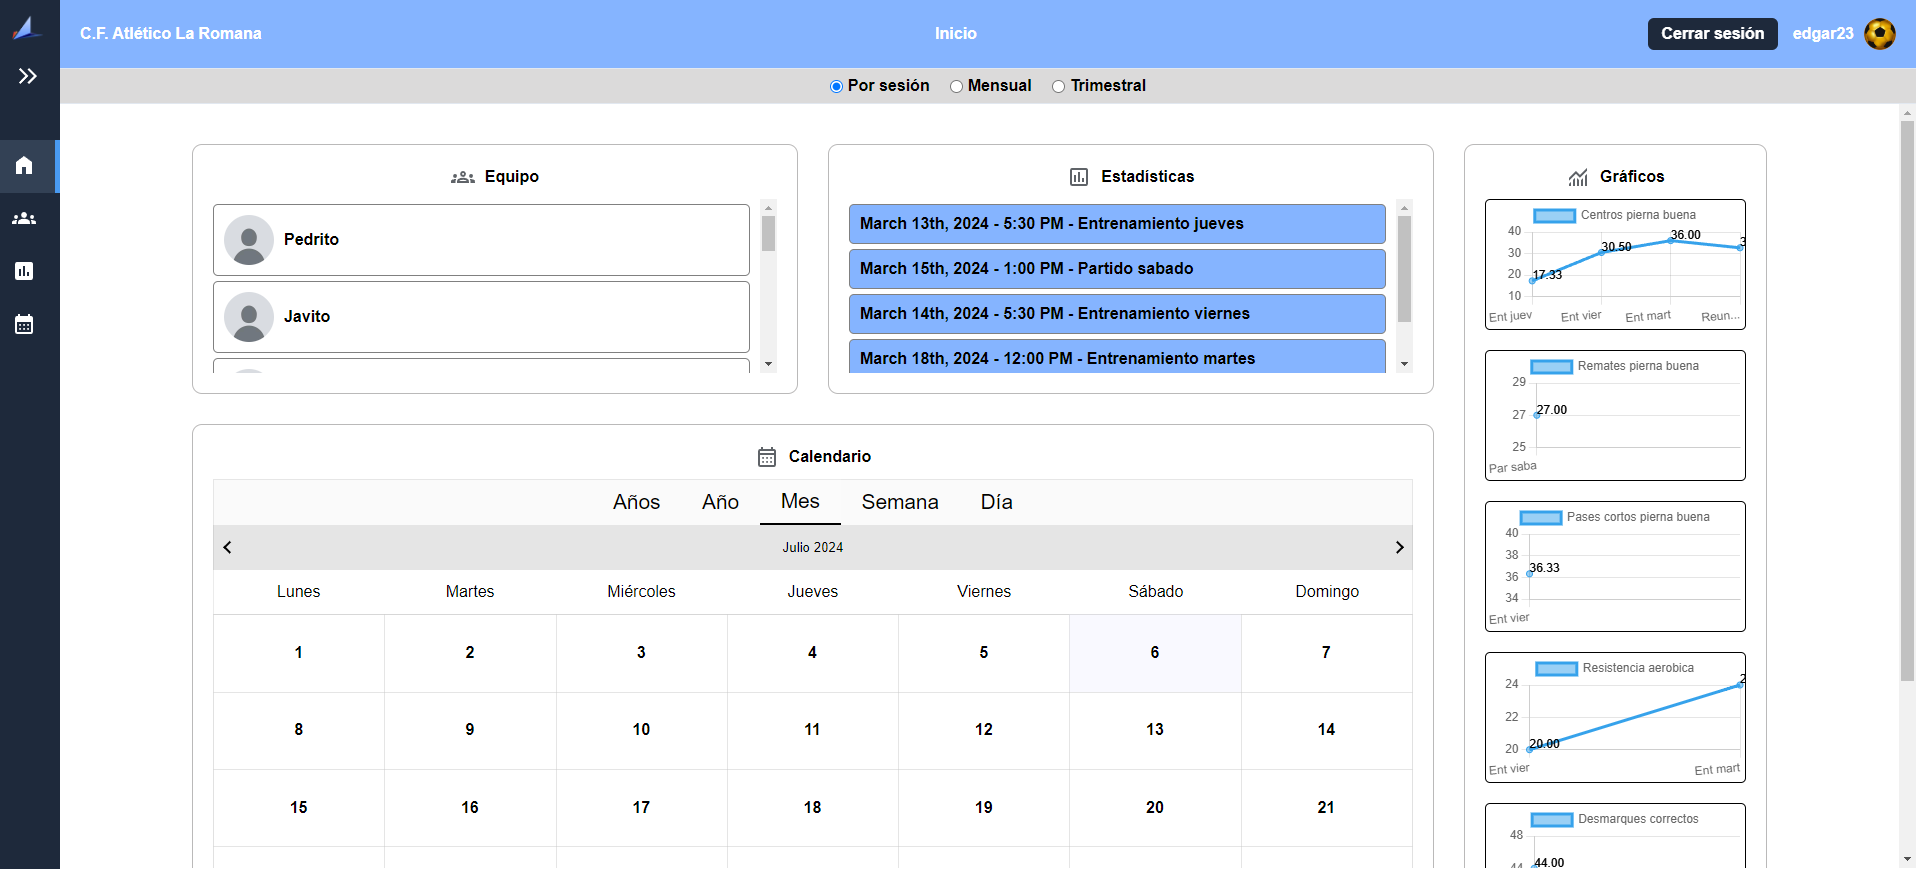
\includegraphics[width=10cm]{archivos/tfg_jorge/pruebas/home_sesion}
    \caption{Ejemplo de la vista principal con el intervalo por sesión seleccionado}\label{sistemass2}
\end{figure}

\begin{figure}[H]
    \centering
    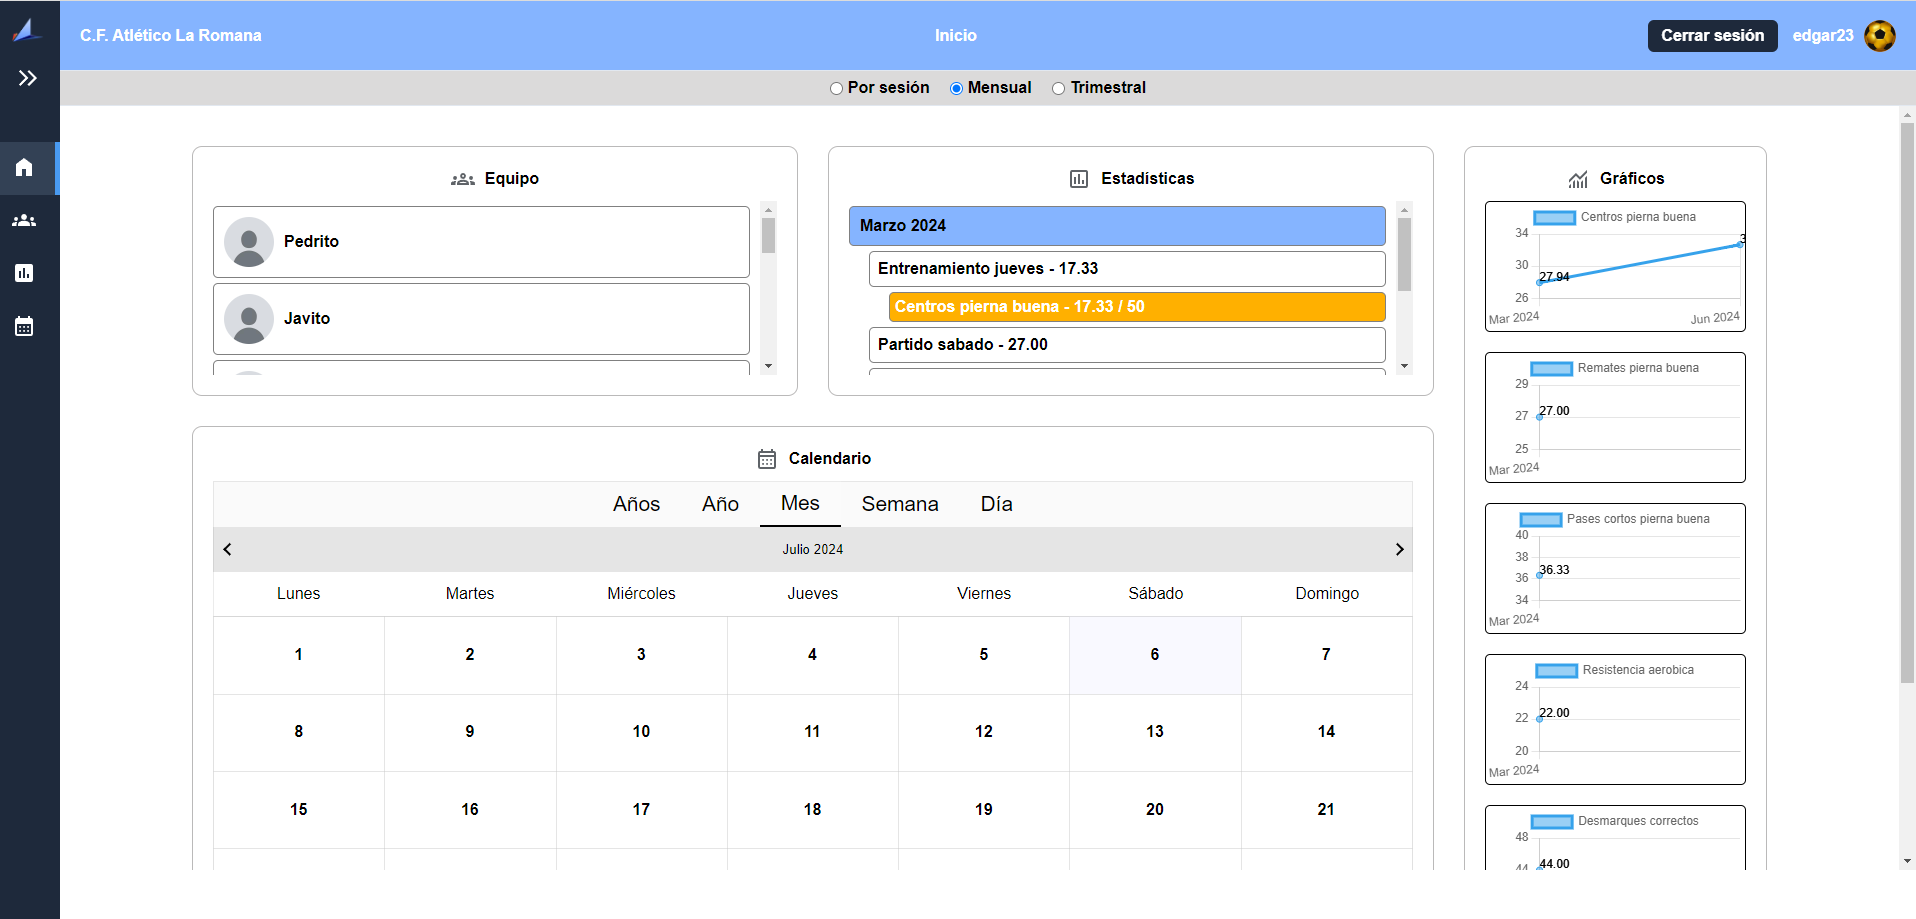
\includegraphics[width=10cm]{archivos/tfg_jorge/pruebas/home_mes}
    \caption{Ejemplo de la vista principal con el intervalo mensual seleccionado}\label{sistemass2}
\end{figure}

\begin{figure}[H]
    \centering
    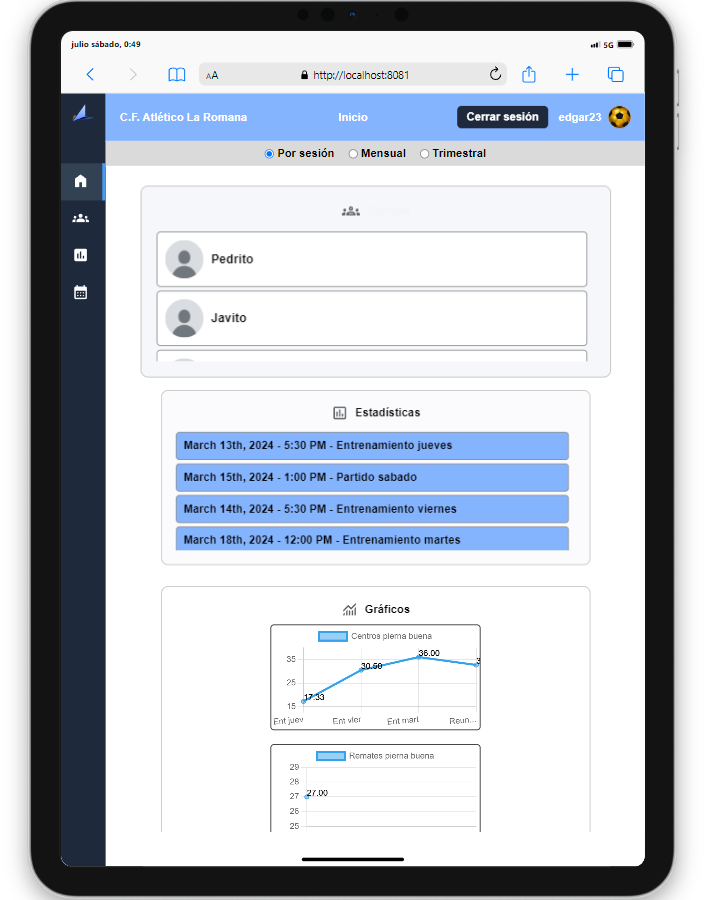
\includegraphics[width=6cm]{archivos/tfg_jorge/pruebas/home_tablet}
    \caption{Vista principal accedida desde una pantalla Ipad 11}\label{sistemass2}
\end{figure}

\begin{figure}[H]
    \centering
    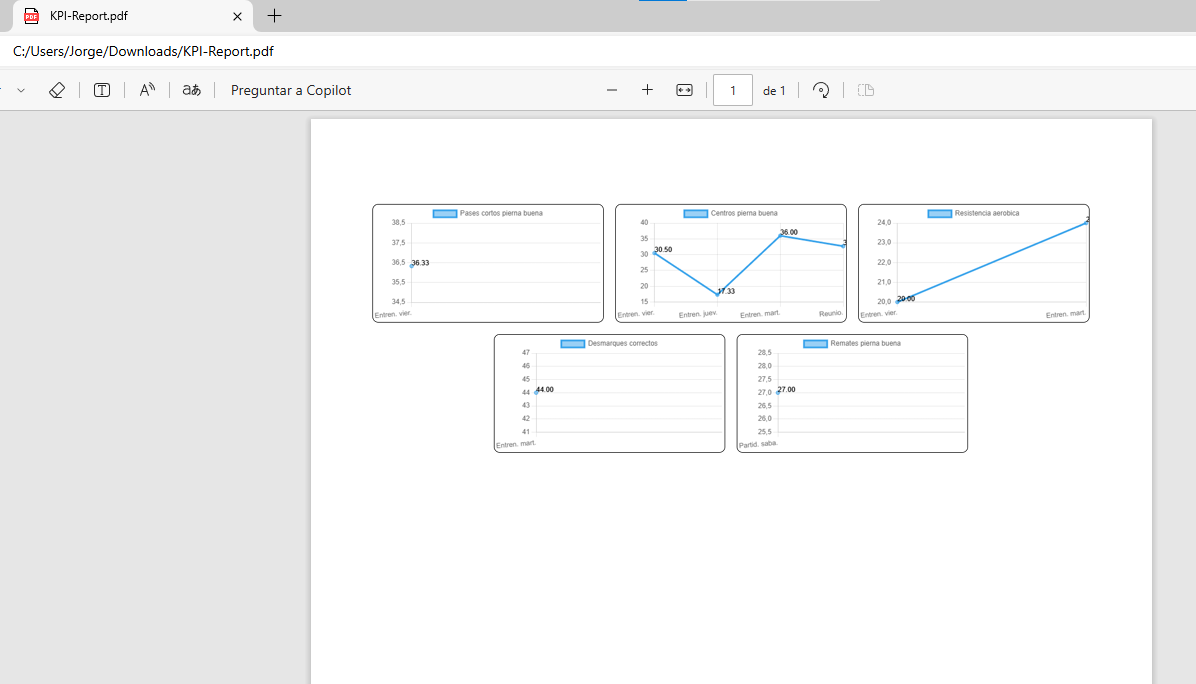
\includegraphics[width=10cm]{archivos/tfg_jorge/pruebas/kpi_report}
    \caption{Informe PDF que se genera desde la vista de estadísticas}\label{sistemass2}
\end{figure}

\begin{figure}[H]
    \centering
    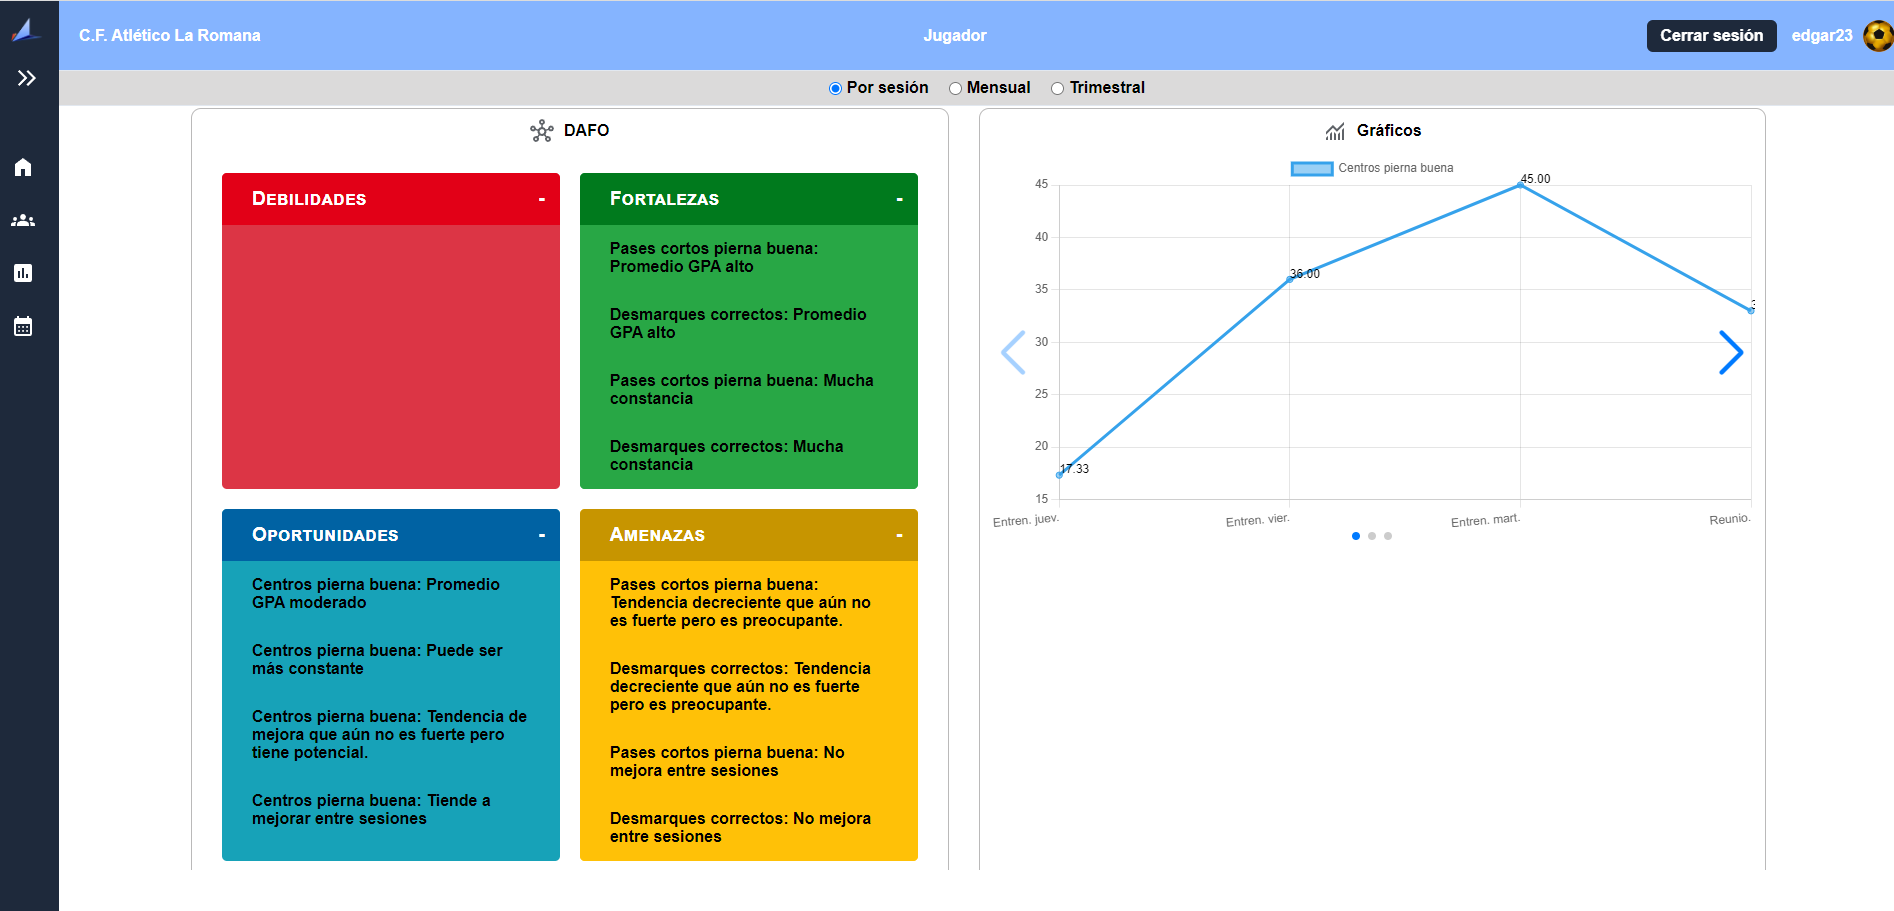
\includegraphics[width=10cm]{archivos/tfg_jorge/pruebas/player_sesion_2}
    \caption{Vista del actor individual con ID 13}\label{sistemass2}
\end{figure}

\begin{figure}[H]
    \centering
    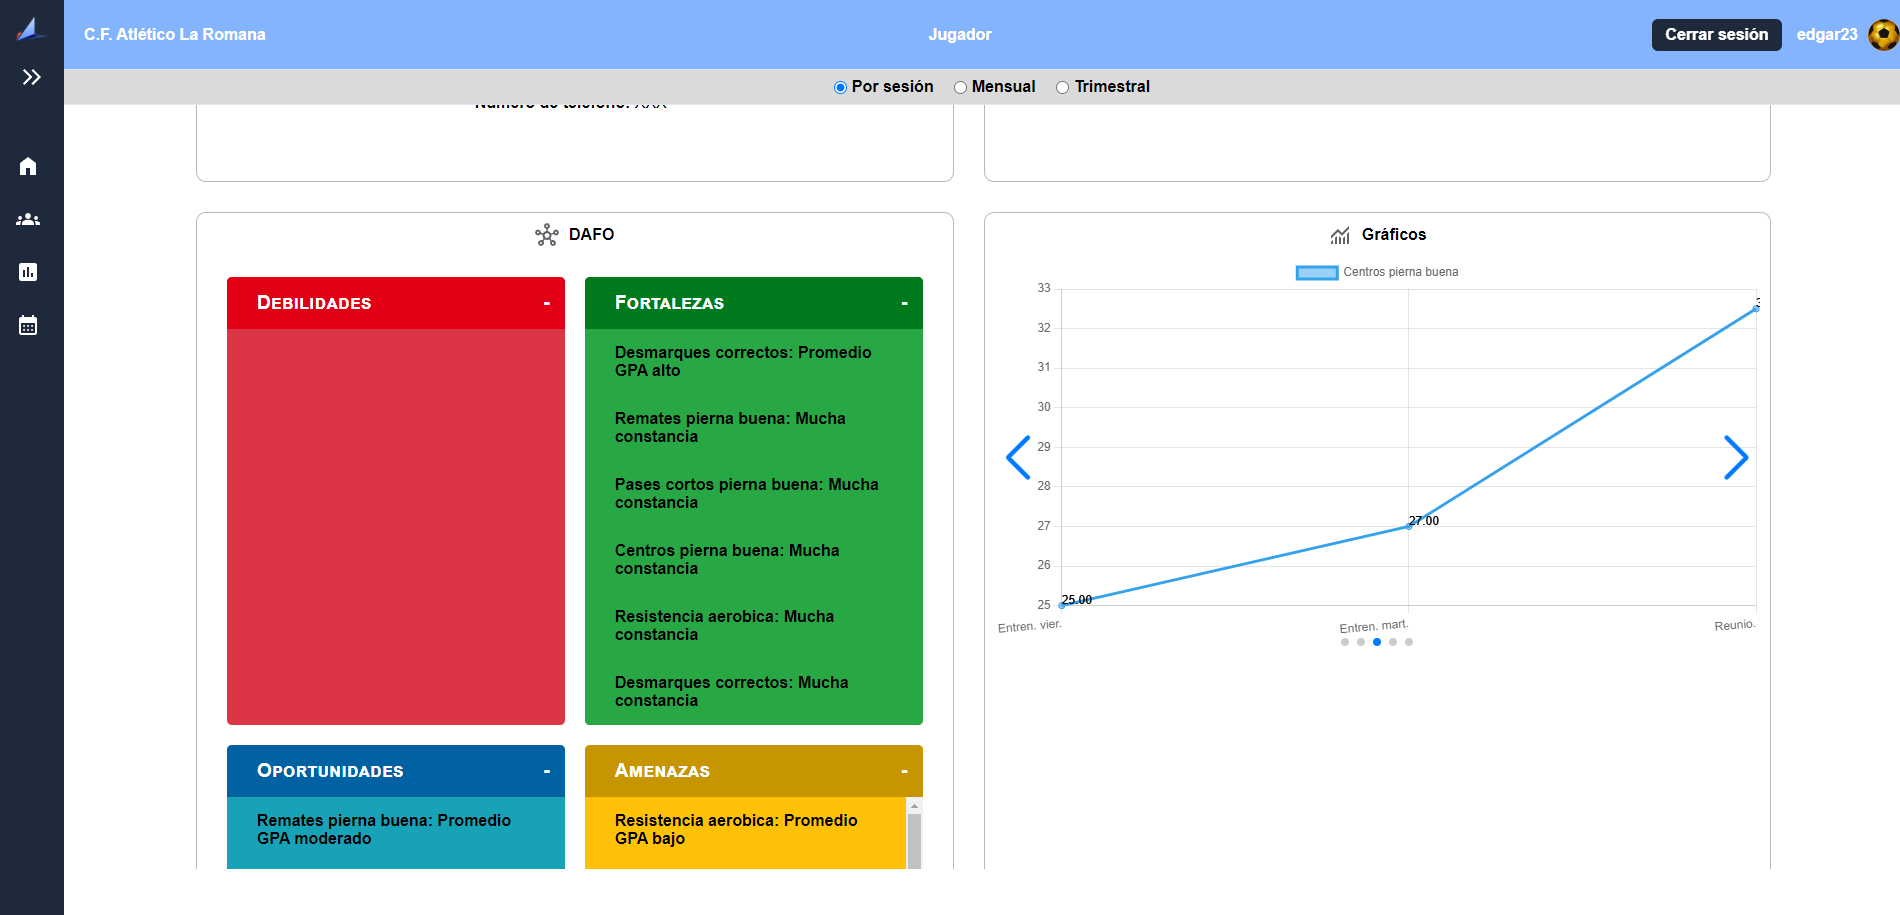
\includegraphics[width=10cm]{archivos/tfg_jorge/pruebas/player_sesion_jugador2}
    \caption{Vista del actor individual con ID 14}\label{sistemass2}
\end{figure}

\begin{figure}[H]
    \centering
    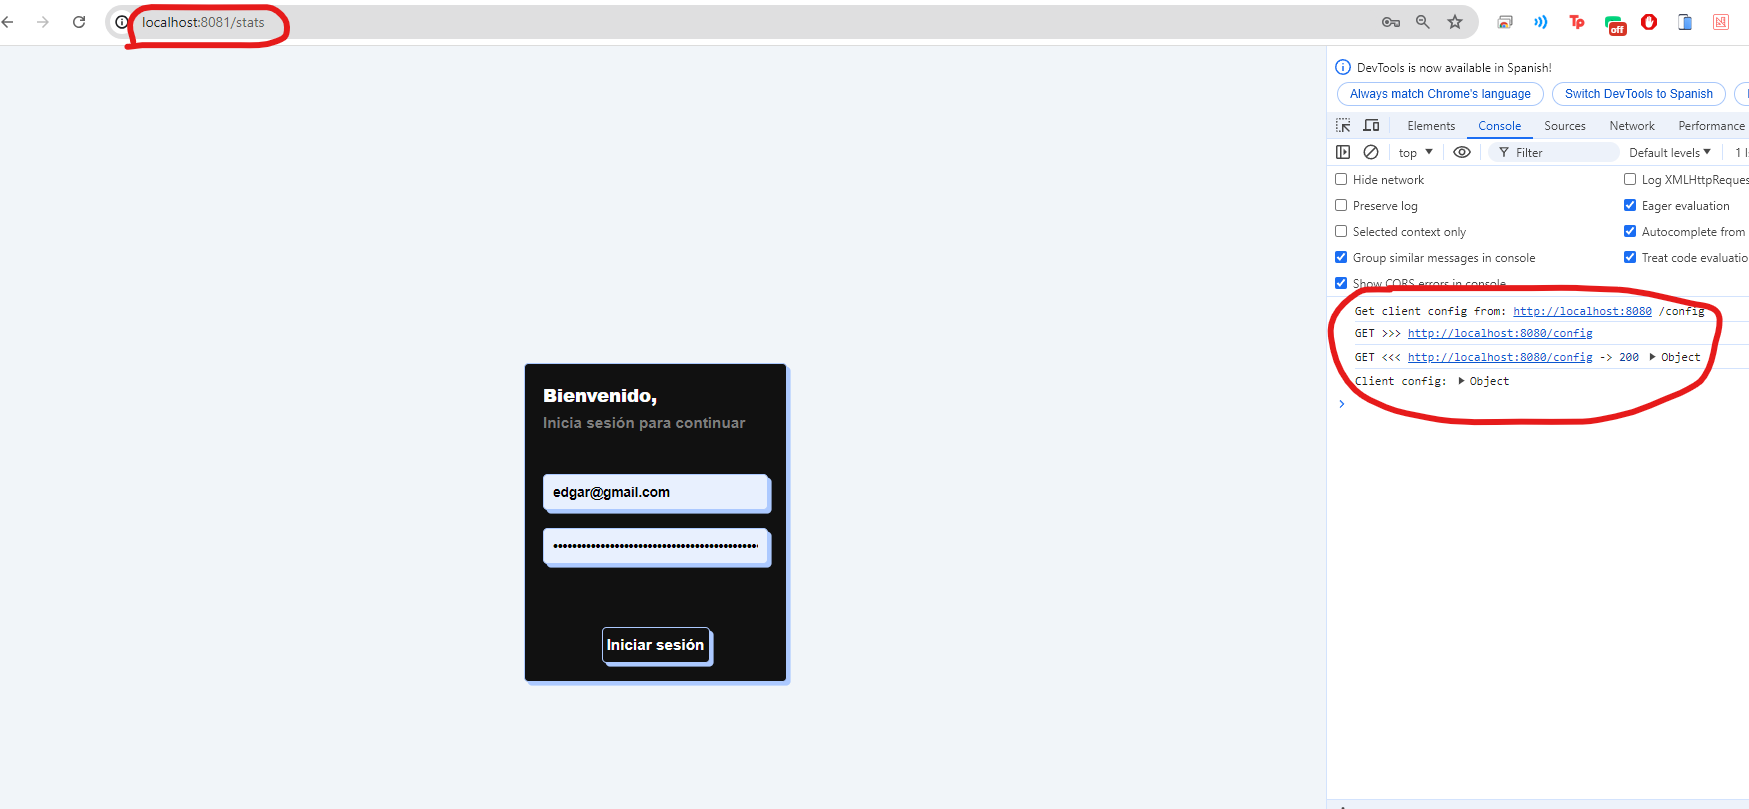
\includegraphics[width=10cm]{archivos/tfg_jorge/pruebas/testAutenticacion}
    \caption{Intento de acceso a URL interna sin haber iniciado sesión}\label{sistemass2}
\end{figure}

\begin{figure}[H]
    \centering
    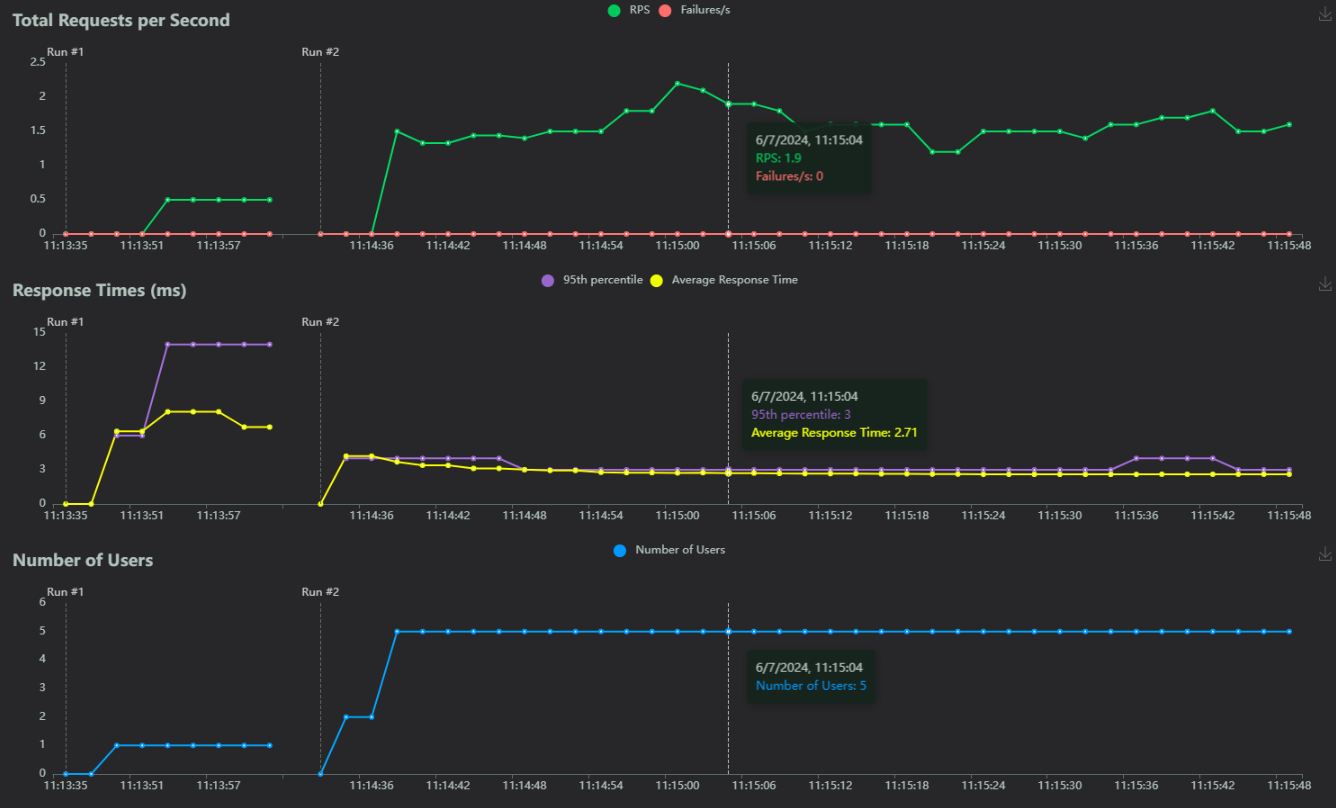
\includegraphics[width=9cm]{archivos/tfg_jorge/pruebas/testRespuesta}
    \caption{Conexiones con múltiples usuarios simultáneos}\label{sistemass2}
\end{figure}
